\documentclass[a4paper]{book}
\usepackage{makeidx}
\usepackage{graphicx}
\usepackage{multicol}
\usepackage{float}
\usepackage{listings}
\usepackage{color}
\usepackage{ifthen}
\usepackage[table]{xcolor}
\usepackage{textcomp}
\usepackage{alltt}
\usepackage{ifpdf}
\ifpdf
\usepackage[pdftex,
            pagebackref=true,
            colorlinks=true,
            linkcolor=blue,
            unicode
           ]{hyperref}
\else
\usepackage[ps2pdf,
            pagebackref=true,
            colorlinks=true,
            linkcolor=blue,
            unicode
           ]{hyperref}
\usepackage{pspicture}
\fi
\usepackage[utf8]{inputenc}
\usepackage{mathptmx}
\usepackage[scaled=.90]{helvet}
\usepackage{courier}
\usepackage{doxygen}
\lstset{language=C++,inputencoding=utf8,basicstyle=\footnotesize,breaklines=true,breakatwhitespace=true,tabsize=8,numbers=left }
\makeindex
\setcounter{tocdepth}{3}
\renewcommand{\footrulewidth}{0.4pt}
\begin{document}
\hypersetup{pageanchor=false}
\begin{titlepage}
\vspace*{7cm}
\begin{center}
{\Large Reference Manual}\\
\vspace*{1cm}
{\large Generated by Doxygen 1.7.3}\\
\vspace*{0.5cm}
{\small Sat Nov 12 2011 20:55:30}\\
\end{center}
\end{titlepage}
\clearemptydoublepage
\pagenumbering{roman}
\tableofcontents
\clearemptydoublepage
\pagenumbering{arabic}
\hypersetup{pageanchor=true}
\chapter{Namespace Index}
\section{Namespace List}
Here is a list of all namespaces with brief descriptions:\begin{DoxyCompactList}
\item\contentsline{section}{\hyperlink{namespacegprof2dot}{gprof2dot} }{\pageref{namespacegprof2dot}}{}
\item\contentsline{section}{\hyperlink{namespacehandlers}{handlers} (Namespace relacionado as funcoes que manipulam interrupcoes de software )}{\pageref{namespacehandlers}}{}
\end{DoxyCompactList}

\chapter{Class Index}
\section{Class Hierarchy}
This inheritance list is sorted roughly, but not completely, alphabetically:\begin{DoxyCompactList}
\item \contentsline{section}{gprof2dot::AQtimeTable}{\pageref{classgprof2dot_1_1AQtimeTable}}{}
\item \contentsline{section}{Builtin}{\pageref{classBuiltin}}{}
\begin{DoxyCompactList}
\item \contentsline{section}{BgCommand}{\pageref{classBgCommand}}{}
\item \contentsline{section}{CdCommand}{\pageref{classCdCommand}}{}
\item \contentsline{section}{ExitCommand}{\pageref{classExitCommand}}{}
\item \contentsline{section}{FgCommand}{\pageref{classFgCommand}}{}
\item \contentsline{section}{JobsCommand}{\pageref{classJobsCommand}}{}
\item \contentsline{section}{KillCommand}{\pageref{classKillCommand}}{}
\item \contentsline{section}{PwdCommand}{\pageref{classPwdCommand}}{}
\end{DoxyCompactList}
\item \contentsline{section}{Command}{\pageref{classCommand}}{}
\item \contentsline{section}{CommandLine}{\pageref{classCommandLine}}{}
\item \contentsline{section}{gprof2dot::DotWriter}{\pageref{classgprof2dot_1_1DotWriter}}{}
\item \contentsline{section}{gprof2dot::Event}{\pageref{classgprof2dot_1_1Event}}{}
\item \contentsline{section}{Executor}{\pageref{classExecutor}}{}
\item \contentsline{section}{Executor::Job}{\pageref{structExecutor_1_1Job}}{}
\item \contentsline{section}{gprof2dot::Main}{\pageref{classgprof2dot_1_1Main}}{}
\item \contentsline{section}{MyTypo}{\pageref{classMyTypo}}{}
\item \contentsline{section}{gprof2dot::Object}{\pageref{classgprof2dot_1_1Object}}{}
\begin{DoxyCompactList}
\item \contentsline{section}{gprof2dot::Call}{\pageref{classgprof2dot_1_1Call}}{}
\item \contentsline{section}{gprof2dot::Cycle}{\pageref{classgprof2dot_1_1Cycle}}{}
\item \contentsline{section}{gprof2dot::Function}{\pageref{classgprof2dot_1_1Function}}{}
\item \contentsline{section}{gprof2dot::Profile}{\pageref{classgprof2dot_1_1Profile}}{}
\end{DoxyCompactList}
\item \contentsline{section}{gprof2dot::ParseError}{\pageref{classgprof2dot_1_1ParseError}}{}
\item \contentsline{section}{Parser}{\pageref{classParser}}{}
\item \contentsline{section}{gprof2dot::Parser}{\pageref{classgprof2dot_1_1Parser}}{}
\begin{DoxyCompactList}
\item \contentsline{section}{gprof2dot::GprofParser}{\pageref{classgprof2dot_1_1GprofParser}}{}
\item \contentsline{section}{gprof2dot::LineParser}{\pageref{classgprof2dot_1_1LineParser}}{}
\begin{DoxyCompactList}
\item \contentsline{section}{gprof2dot::CallgrindParser}{\pageref{classgprof2dot_1_1CallgrindParser}}{}
\item \contentsline{section}{gprof2dot::HProfParser}{\pageref{classgprof2dot_1_1HProfParser}}{}
\item \contentsline{section}{gprof2dot::OprofileParser}{\pageref{classgprof2dot_1_1OprofileParser}}{}
\item \contentsline{section}{gprof2dot::PerfParser}{\pageref{classgprof2dot_1_1PerfParser}}{}
\item \contentsline{section}{gprof2dot::SharkParser}{\pageref{classgprof2dot_1_1SharkParser}}{}
\end{DoxyCompactList}
\item \contentsline{section}{gprof2dot::SleepyParser}{\pageref{classgprof2dot_1_1SleepyParser}}{}
\item \contentsline{section}{gprof2dot::XmlParser}{\pageref{classgprof2dot_1_1XmlParser}}{}
\begin{DoxyCompactList}
\item \contentsline{section}{gprof2dot::AQtimeParser}{\pageref{classgprof2dot_1_1AQtimeParser}}{}
\item \contentsline{section}{gprof2dot::SysprofParser}{\pageref{classgprof2dot_1_1SysprofParser}}{}
\end{DoxyCompactList}
\item \contentsline{section}{gprof2dot::XPerfParser}{\pageref{classgprof2dot_1_1XPerfParser}}{}
\end{DoxyCompactList}
\item \contentsline{section}{Program}{\pageref{classProgram}}{}
\item \contentsline{section}{gprof2dot::PstatsParser}{\pageref{classgprof2dot_1_1PstatsParser}}{}
\item \contentsline{section}{gprof2dot::Struct}{\pageref{classgprof2dot_1_1Struct}}{}
\item \contentsline{section}{gprof2dot::Theme}{\pageref{classgprof2dot_1_1Theme}}{}
\item \contentsline{section}{gprof2dot::UndefinedEvent}{\pageref{classgprof2dot_1_1UndefinedEvent}}{}
\item \contentsline{section}{gprof2dot::XmlToken}{\pageref{classgprof2dot_1_1XmlToken}}{}
\item \contentsline{section}{gprof2dot::XmlTokenizer}{\pageref{classgprof2dot_1_1XmlTokenizer}}{}
\item \contentsline{section}{gprof2dot::XmlTokenMismatch}{\pageref{classgprof2dot_1_1XmlTokenMismatch}}{}
\end{DoxyCompactList}

\chapter{Class Index}
\section{Class List}
Here are the classes, structs, unions and interfaces with brief descriptions:\begin{DoxyCompactList}
\item\contentsline{section}{\hyperlink{classgprof2dot_1_1AQtimeParser}{gprof2dot::AQtimeParser} }{\pageref{classgprof2dot_1_1AQtimeParser}}{}
\item\contentsline{section}{\hyperlink{classgprof2dot_1_1AQtimeTable}{gprof2dot::AQtimeTable} }{\pageref{classgprof2dot_1_1AQtimeTable}}{}
\item\contentsline{section}{\hyperlink{classBgCommand}{BgCommand} (Classe que implementa o comando bg )}{\pageref{classBgCommand}}{}
\item\contentsline{section}{\hyperlink{classBuiltin}{Builtin} (Classe abstrata para comandos Built-\/In )}{\pageref{classBuiltin}}{}
\item\contentsline{section}{\hyperlink{classgprof2dot_1_1Call}{gprof2dot::Call} }{\pageref{classgprof2dot_1_1Call}}{}
\item\contentsline{section}{\hyperlink{classgprof2dot_1_1CallgrindParser}{gprof2dot::CallgrindParser} }{\pageref{classgprof2dot_1_1CallgrindParser}}{}
\item\contentsline{section}{\hyperlink{classCdCommand}{CdCommand} (Classe que implementa o comando cd )}{\pageref{classCdCommand}}{}
\item\contentsline{section}{\hyperlink{classCommand}{Command} (Representa um comando entrado pelo usuario. O comando representa tudo o que esta antes de um pipe ( $|$ ) ou \& ou final de linha )}{\pageref{classCommand}}{}
\item\contentsline{section}{\hyperlink{classCommandLine}{CommandLine} (Represeta uma linha de comando )}{\pageref{classCommandLine}}{}
\item\contentsline{section}{\hyperlink{classgprof2dot_1_1Cycle}{gprof2dot::Cycle} }{\pageref{classgprof2dot_1_1Cycle}}{}
\item\contentsline{section}{\hyperlink{classgprof2dot_1_1DotWriter}{gprof2dot::DotWriter} }{\pageref{classgprof2dot_1_1DotWriter}}{}
\item\contentsline{section}{\hyperlink{classgprof2dot_1_1Event}{gprof2dot::Event} }{\pageref{classgprof2dot_1_1Event}}{}
\item\contentsline{section}{\hyperlink{classExecutor}{Executor} (Responsavel pela execucao. Executa uma linha de comando )}{\pageref{classExecutor}}{}
\item\contentsline{section}{\hyperlink{classExitCommand}{ExitCommand} (Classe que implementa o comando exit )}{\pageref{classExitCommand}}{}
\item\contentsline{section}{\hyperlink{classFgCommand}{FgCommand} (Classe que implementa o comando fg )}{\pageref{classFgCommand}}{}
\item\contentsline{section}{\hyperlink{classgprof2dot_1_1Function}{gprof2dot::Function} }{\pageref{classgprof2dot_1_1Function}}{}
\item\contentsline{section}{\hyperlink{classgprof2dot_1_1GprofParser}{gprof2dot::GprofParser} }{\pageref{classgprof2dot_1_1GprofParser}}{}
\item\contentsline{section}{\hyperlink{classgprof2dot_1_1HProfParser}{gprof2dot::HProfParser} }{\pageref{classgprof2dot_1_1HProfParser}}{}
\item\contentsline{section}{\hyperlink{structExecutor_1_1Job}{Executor::Job} (Estrutura que representa um job. Guarda os dados necessarios para controlar processos )}{\pageref{structExecutor_1_1Job}}{}
\item\contentsline{section}{\hyperlink{classJobsCommand}{JobsCommand} (Classe que implementa o comando jobs )}{\pageref{classJobsCommand}}{}
\item\contentsline{section}{\hyperlink{classKillCommand}{KillCommand} (Classe que implementa o comando kill )}{\pageref{classKillCommand}}{}
\item\contentsline{section}{\hyperlink{classgprof2dot_1_1LineParser}{gprof2dot::LineParser} }{\pageref{classgprof2dot_1_1LineParser}}{}
\item\contentsline{section}{\hyperlink{classgprof2dot_1_1Main}{gprof2dot::Main} }{\pageref{classgprof2dot_1_1Main}}{}
\item\contentsline{section}{\hyperlink{classMyTypo}{MyTypo} (Firulas )}{\pageref{classMyTypo}}{}
\item\contentsline{section}{\hyperlink{classgprof2dot_1_1Object}{gprof2dot::Object} }{\pageref{classgprof2dot_1_1Object}}{}
\item\contentsline{section}{\hyperlink{classgprof2dot_1_1OprofileParser}{gprof2dot::OprofileParser} }{\pageref{classgprof2dot_1_1OprofileParser}}{}
\item\contentsline{section}{\hyperlink{classgprof2dot_1_1ParseError}{gprof2dot::ParseError} }{\pageref{classgprof2dot_1_1ParseError}}{}
\item\contentsline{section}{\hyperlink{classParser}{Parser} (Utilizado para converter a entrada do usuario em uma \hyperlink{classCommandLine}{CommandLine} )}{\pageref{classParser}}{}
\item\contentsline{section}{\hyperlink{classgprof2dot_1_1Parser}{gprof2dot::Parser} }{\pageref{classgprof2dot_1_1Parser}}{}
\item\contentsline{section}{\hyperlink{classgprof2dot_1_1PerfParser}{gprof2dot::PerfParser} }{\pageref{classgprof2dot_1_1PerfParser}}{}
\item\contentsline{section}{\hyperlink{classgprof2dot_1_1Profile}{gprof2dot::Profile} }{\pageref{classgprof2dot_1_1Profile}}{}
\item\contentsline{section}{\hyperlink{classProgram}{Program} }{\pageref{classProgram}}{}
\item\contentsline{section}{\hyperlink{classgprof2dot_1_1PstatsParser}{gprof2dot::PstatsParser} }{\pageref{classgprof2dot_1_1PstatsParser}}{}
\item\contentsline{section}{\hyperlink{classPwdCommand}{PwdCommand} (Classe que implementa o comando pwd )}{\pageref{classPwdCommand}}{}
\item\contentsline{section}{\hyperlink{classgprof2dot_1_1SharkParser}{gprof2dot::SharkParser} }{\pageref{classgprof2dot_1_1SharkParser}}{}
\item\contentsline{section}{\hyperlink{classgprof2dot_1_1SleepyParser}{gprof2dot::SleepyParser} }{\pageref{classgprof2dot_1_1SleepyParser}}{}
\item\contentsline{section}{\hyperlink{classgprof2dot_1_1Struct}{gprof2dot::Struct} }{\pageref{classgprof2dot_1_1Struct}}{}
\item\contentsline{section}{\hyperlink{classgprof2dot_1_1SysprofParser}{gprof2dot::SysprofParser} }{\pageref{classgprof2dot_1_1SysprofParser}}{}
\item\contentsline{section}{\hyperlink{classgprof2dot_1_1Theme}{gprof2dot::Theme} }{\pageref{classgprof2dot_1_1Theme}}{}
\item\contentsline{section}{\hyperlink{classgprof2dot_1_1UndefinedEvent}{gprof2dot::UndefinedEvent} }{\pageref{classgprof2dot_1_1UndefinedEvent}}{}
\item\contentsline{section}{\hyperlink{classgprof2dot_1_1XmlParser}{gprof2dot::XmlParser} }{\pageref{classgprof2dot_1_1XmlParser}}{}
\item\contentsline{section}{\hyperlink{classgprof2dot_1_1XmlToken}{gprof2dot::XmlToken} }{\pageref{classgprof2dot_1_1XmlToken}}{}
\item\contentsline{section}{\hyperlink{classgprof2dot_1_1XmlTokenizer}{gprof2dot::XmlTokenizer} }{\pageref{classgprof2dot_1_1XmlTokenizer}}{}
\item\contentsline{section}{\hyperlink{classgprof2dot_1_1XmlTokenMismatch}{gprof2dot::XmlTokenMismatch} }{\pageref{classgprof2dot_1_1XmlTokenMismatch}}{}
\item\contentsline{section}{\hyperlink{classgprof2dot_1_1XPerfParser}{gprof2dot::XPerfParser} }{\pageref{classgprof2dot_1_1XPerfParser}}{}
\end{DoxyCompactList}

\chapter{File Index}
\section{File List}
Here is a list of all files with brief descriptions:\begin{DoxyCompactList}
\item\contentsline{section}{\hyperlink{Builtin_8cpp}{Builtin.cpp} }{\pageref{Builtin_8cpp}}{}
\item\contentsline{section}{\hyperlink{Builtin_8hpp}{Builtin.hpp} }{\pageref{Builtin_8hpp}}{}
\item\contentsline{section}{\hyperlink{Command_8cpp}{Command.cpp} }{\pageref{Command_8cpp}}{}
\item\contentsline{section}{\hyperlink{Command_8hpp}{Command.hpp} }{\pageref{Command_8hpp}}{}
\item\contentsline{section}{\hyperlink{CommandLine_8cpp}{CommandLine.cpp} }{\pageref{CommandLine_8cpp}}{}
\item\contentsline{section}{\hyperlink{CommandLine_8hpp}{CommandLine.hpp} }{\pageref{CommandLine_8hpp}}{}
\item\contentsline{section}{\hyperlink{Executor_8cpp}{Executor.cpp} }{\pageref{Executor_8cpp}}{}
\item\contentsline{section}{\hyperlink{Executor_8hpp}{Executor.hpp} }{\pageref{Executor_8hpp}}{}
\item\contentsline{section}{\hyperlink{gprof2dot_8py}{gprof2dot.py} }{\pageref{gprof2dot_8py}}{}
\item\contentsline{section}{\hyperlink{Handlers_8cpp}{Handlers.cpp} }{\pageref{Handlers_8cpp}}{}
\item\contentsline{section}{\hyperlink{Handlers_8hpp}{Handlers.hpp} }{\pageref{Handlers_8hpp}}{}
\item\contentsline{section}{\hyperlink{main_8cpp}{main.cpp} }{\pageref{main_8cpp}}{}
\item\contentsline{section}{\hyperlink{MyTypo_8cpp}{MyTypo.cpp} }{\pageref{MyTypo_8cpp}}{}
\item\contentsline{section}{\hyperlink{MyTypo_8hpp}{MyTypo.hpp} }{\pageref{MyTypo_8hpp}}{}
\item\contentsline{section}{\hyperlink{Parser_8cpp}{Parser.cpp} }{\pageref{Parser_8cpp}}{}
\item\contentsline{section}{\hyperlink{Parser_8hpp}{Parser.hpp} }{\pageref{Parser_8hpp}}{}
\item\contentsline{section}{\hyperlink{Program_8cpp}{Program.cpp} }{\pageref{Program_8cpp}}{}
\item\contentsline{section}{\hyperlink{Program_8hpp}{Program.hpp} }{\pageref{Program_8hpp}}{}
\end{DoxyCompactList}

\chapter{Namespace Documentation}
\hypertarget{namespacehandlers}{
\section{handlers Namespace Reference}
\label{namespacehandlers}\index{handlers@{handlers}}
}


Namespace relacionado as funcoes que manipulam interrupcoes de software.  


\subsection*{Functions}
\begin{DoxyCompactItemize}
\item 
void \hyperlink{namespacehandlers_aa02fd1a028b7cfc01ccb52b9f70cb624}{sigChildHandler} (int)
\begin{DoxyCompactList}\small\item\em Handler para o sinal SIGCHLD. Levanta uma flag dizendo que um sinal vindo de um provesso filho foi lancado. \item\end{DoxyCompactList}\item 
bool \hyperlink{namespacehandlers_a7f732d800eb51bf0ee24d554ce770276}{getDeathStatus} ()
\item 
void \hyperlink{namespacehandlers_a254dfa6abeed4136e566fd013aa9fdc4}{setDeathStatusFalse} ()
\begin{DoxyCompactList}\small\item\em Altera a flag de sinais recebidos. Altera o valor da flag de sinais recebidos para false. \item\end{DoxyCompactList}\item 
void \hyperlink{namespacehandlers_a06dc78ff46f5dcc7fb9c09a495caf4ff}{setDeathStatusTrue} ()
\begin{DoxyCompactList}\small\item\em Altera a flag de sinais recebidos. Altera o valor da flag de sinais recebidos para true. \item\end{DoxyCompactList}\end{DoxyCompactItemize}


\subsection{Detailed Description}
Namespace relacionado as funcoes que manipulam interrupcoes de software. 

\subsection{Function Documentation}
\hypertarget{namespacehandlers_a7f732d800eb51bf0ee24d554ce770276}{
\index{handlers@{handlers}!getDeathStatus@{getDeathStatus}}
\index{getDeathStatus@{getDeathStatus}!handlers@{handlers}}
\subsubsection[{getDeathStatus}]{\setlength{\rightskip}{0pt plus 5cm}bool handlers::getDeathStatus (
\begin{DoxyParamCaption}
{}
\end{DoxyParamCaption}
)}}
\label{namespacehandlers_a7f732d800eb51bf0ee24d554ce770276}
\begin{DoxyReturn}{Returns}
Retorna se ha novos sinais para serem processados. 
\end{DoxyReturn}
\hypertarget{namespacehandlers_a254dfa6abeed4136e566fd013aa9fdc4}{
\index{handlers@{handlers}!setDeathStatusFalse@{setDeathStatusFalse}}
\index{setDeathStatusFalse@{setDeathStatusFalse}!handlers@{handlers}}
\subsubsection[{setDeathStatusFalse}]{\setlength{\rightskip}{0pt plus 5cm}void handlers::setDeathStatusFalse (
\begin{DoxyParamCaption}
{}
\end{DoxyParamCaption}
)}}
\label{namespacehandlers_a254dfa6abeed4136e566fd013aa9fdc4}


Altera a flag de sinais recebidos. Altera o valor da flag de sinais recebidos para false. 

\hypertarget{namespacehandlers_a06dc78ff46f5dcc7fb9c09a495caf4ff}{
\index{handlers@{handlers}!setDeathStatusTrue@{setDeathStatusTrue}}
\index{setDeathStatusTrue@{setDeathStatusTrue}!handlers@{handlers}}
\subsubsection[{setDeathStatusTrue}]{\setlength{\rightskip}{0pt plus 5cm}void handlers::setDeathStatusTrue (
\begin{DoxyParamCaption}
{}
\end{DoxyParamCaption}
)}}
\label{namespacehandlers_a06dc78ff46f5dcc7fb9c09a495caf4ff}


Altera a flag de sinais recebidos. Altera o valor da flag de sinais recebidos para true. 

\hypertarget{namespacehandlers_aa02fd1a028b7cfc01ccb52b9f70cb624}{
\index{handlers@{handlers}!sigChildHandler@{sigChildHandler}}
\index{sigChildHandler@{sigChildHandler}!handlers@{handlers}}
\subsubsection[{sigChildHandler}]{\setlength{\rightskip}{0pt plus 5cm}void handlers::sigChildHandler (
\begin{DoxyParamCaption}
\item[{int}]{signum}
\end{DoxyParamCaption}
)}}
\label{namespacehandlers_aa02fd1a028b7cfc01ccb52b9f70cb624}


Handler para o sinal SIGCHLD. Levanta uma flag dizendo que um sinal vindo de um provesso filho foi lancado. 


\chapter{Class Documentation}
\hypertarget{classBgCommand}{
\section{BgCommand Class Reference}
\label{classBgCommand}\index{BgCommand@{BgCommand}}
}


Classe que implementa o comando bg.  




{\ttfamily \#include $<$Builtin.hpp$>$}

Inheritance diagram for BgCommand:\begin{figure}[H]
\begin{center}
\leavevmode
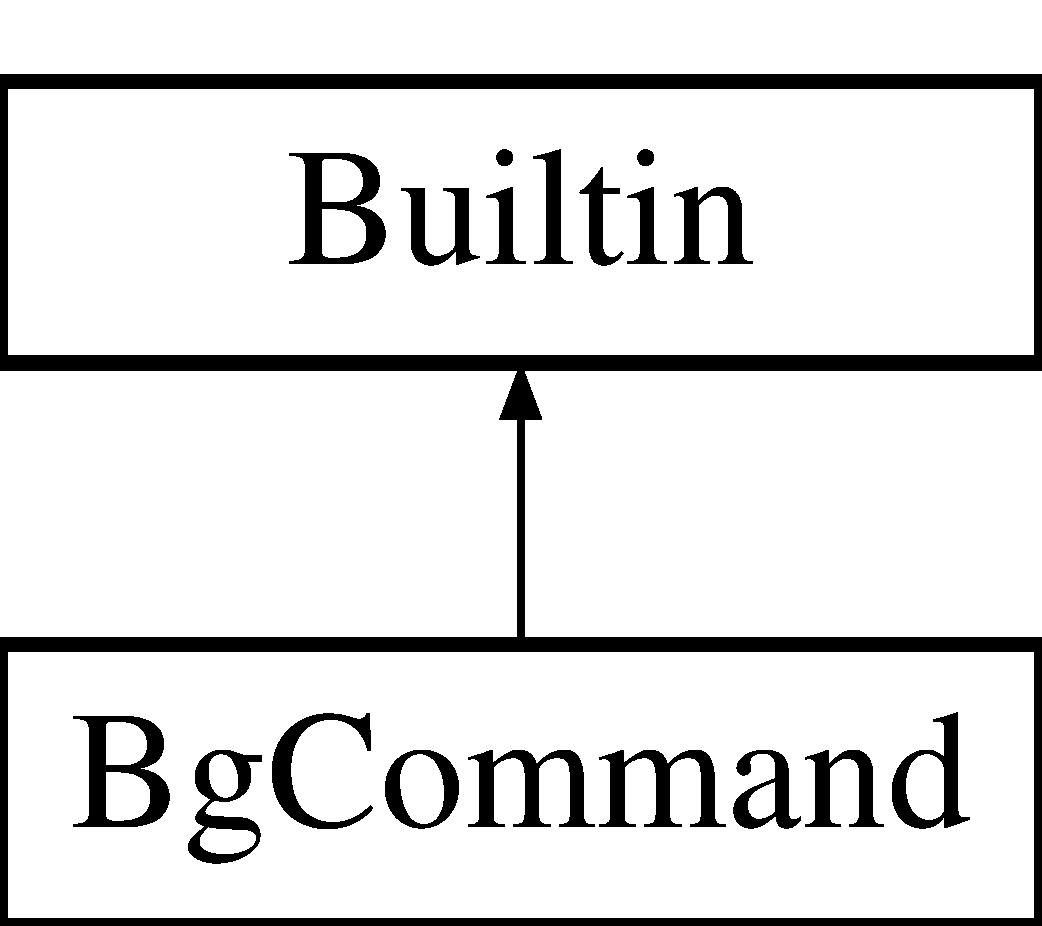
\includegraphics[height=2.000000cm]{classBgCommand}
\end{center}
\end{figure}


\subsection{Detailed Description}
Classe que implementa o comando bg. Sintaxe: bg \%$<$JOBID$>$ $|$ bg\par
 Se o comando for chamado sem o JOBID, sera utilizado o job mais recentemente aberto, colocado em foreground ou background ou, caso ja tenha sido fechado, o mais antigo aberto. 

The documentation for this class was generated from the following files:\begin{DoxyCompactItemize}
\item 
\hyperlink{Builtin_8hpp}{Builtin.hpp}\item 
\hyperlink{Builtin_8cpp}{Builtin.cpp}\end{DoxyCompactItemize}

\hypertarget{classBuiltin}{
\section{Builtin Class Reference}
\label{classBuiltin}\index{Builtin@{Builtin}}
}


{\ttfamily \#include $<$Builtin.hpp$>$}

Inheritance diagram for Builtin:\begin{figure}[H]
\begin{center}
\leavevmode
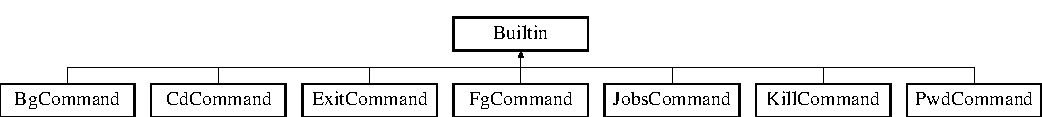
\includegraphics[height=1.568627cm]{classBuiltin}
\end{center}
\end{figure}
\subsection*{Public Member Functions}
\begin{DoxyCompactItemize}
\item 
void \hyperlink{classBuiltin_aeb4e6144d47e07c4afedb20ee66671be}{run} (const char $\ast$\mbox{[}$\,$\mbox{]}, \hyperlink{classExecutor}{Executor} $\ast$)
\item 
virtual bool \hyperlink{classBuiltin_a91ec773bbed5e1a8808955d9b48e664b}{forkable} ()
\end{DoxyCompactItemize}


\subsection{Member Function Documentation}
\hypertarget{classBuiltin_a91ec773bbed5e1a8808955d9b48e664b}{
\index{Builtin@{Builtin}!forkable@{forkable}}
\index{forkable@{forkable}!Builtin@{Builtin}}
\subsubsection[{forkable}]{\setlength{\rightskip}{0pt plus 5cm}bool Builtin::forkable (
\begin{DoxyParamCaption}
{}
\end{DoxyParamCaption}
)\hspace{0.3cm}{\ttfamily  \mbox{[}virtual\mbox{]}}}}
\label{classBuiltin_a91ec773bbed5e1a8808955d9b48e664b}
\hypertarget{classBuiltin_aeb4e6144d47e07c4afedb20ee66671be}{
\index{Builtin@{Builtin}!run@{run}}
\index{run@{run}!Builtin@{Builtin}}
\subsubsection[{run}]{\setlength{\rightskip}{0pt plus 5cm}void Builtin::run (
\begin{DoxyParamCaption}
\item[{const char $\ast$}]{args\mbox{[}$\,$\mbox{]}, }
\item[{{\bf Executor} $\ast$}]{executor}
\end{DoxyParamCaption}
)}}
\label{classBuiltin_aeb4e6144d47e07c4afedb20ee66671be}


The documentation for this class was generated from the following files:\begin{DoxyCompactItemize}
\item 
\hyperlink{Builtin_8hpp}{Builtin.hpp}\item 
\hyperlink{Builtin_8cpp}{Builtin.cpp}\end{DoxyCompactItemize}

\hypertarget{classCdCommand}{
\section{CdCommand Class Reference}
\label{classCdCommand}\index{CdCommand@{CdCommand}}
}


Classe que implementa o comando cd.  




{\ttfamily \#include $<$Builtin.hpp$>$}

Inheritance diagram for CdCommand:\begin{figure}[H]
\begin{center}
\leavevmode
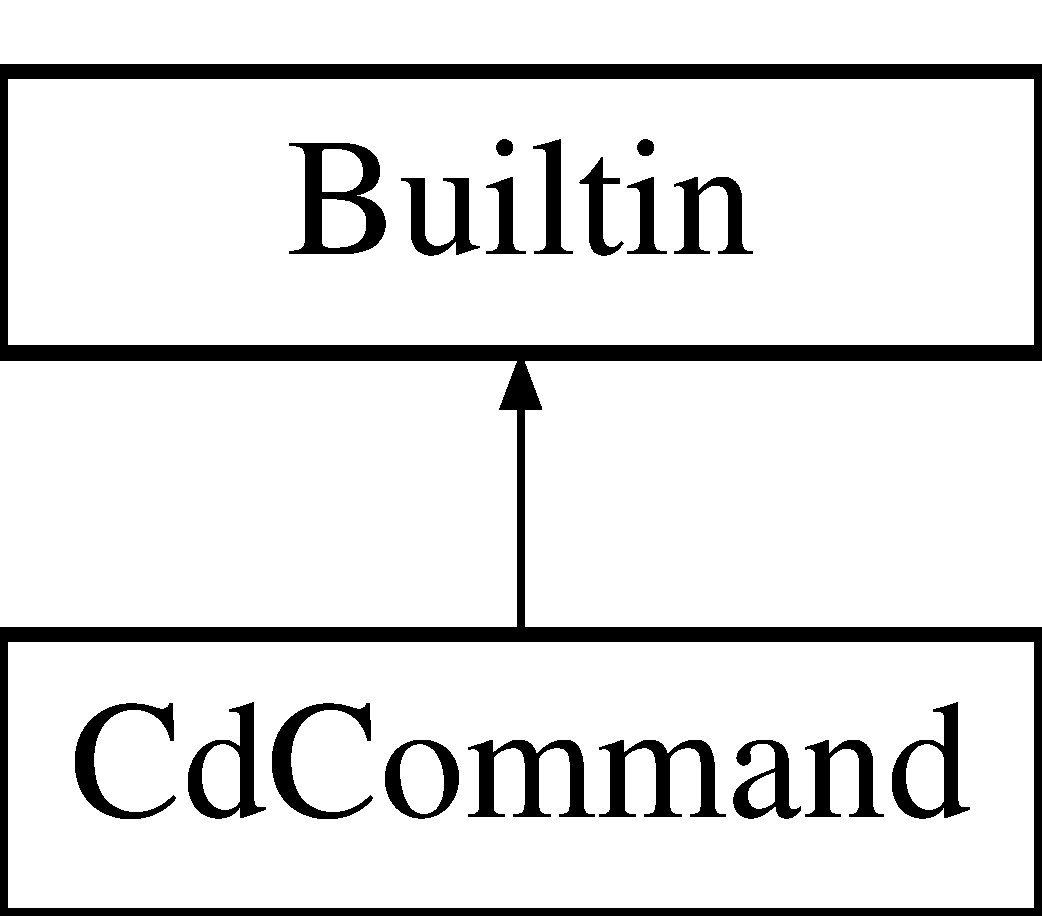
\includegraphics[height=2.000000cm]{classCdCommand}
\end{center}
\end{figure}


\subsection{Detailed Description}
Classe que implementa o comando cd. Sintaxe: cd $<$diretorio$>$ 

The documentation for this class was generated from the following files:\begin{DoxyCompactItemize}
\item 
\hyperlink{Builtin_8hpp}{Builtin.hpp}\item 
\hyperlink{Builtin_8cpp}{Builtin.cpp}\end{DoxyCompactItemize}

\hypertarget{classCommand}{
\section{Command Class Reference}
\label{classCommand}\index{Command@{Command}}
}


Representa um comando entrado pelo usuario. O comando representa tudo que esta numa linha ou antes de um \&.  




{\ttfamily \#include $<$Command.hpp$>$}

\subsection*{Public Member Functions}
\begin{DoxyCompactItemize}
\item 
\hyperlink{classCommand_a649b404d34720e098d6e0de6b07ad0c1}{Command} (std::vector$<$ std::string $>$ \&parameters, std::string in=std::string(), std::string out=std::string(), std::string err=std::string(), bool outAppend=false, bool errAppend=false)
\item 
\hyperlink{classCommand_ab552bb3a07fdd1acbfd8ea76e69b2278}{$\sim$Command} ()
\item 
std::string \hyperlink{classCommand_a660ad6733da715bcd5f74a38c04f4527}{getIn} ()
\item 
std::string \hyperlink{classCommand_a63ab07191770dd7f8133e49f8c4552d6}{getOut} ()
\item 
std::string \hyperlink{classCommand_a0421ff1ec0e2aec12fe8a334ceaea3ef}{getErr} ()
\item 
bool \hyperlink{classCommand_a054da0acd3b09e33c40df6865fc29c55}{getOutAppend} ()
\item 
bool \hyperlink{classCommand_a59a9ec8f011e3467e36ad72a8bcd3129}{getErrAppend} ()
\item 
const char $\ast$$\ast$ \hyperlink{classCommand_a37ef9c4ef69e9de78c138b0fe6b98f9f}{getExecv} ()
\end{DoxyCompactItemize}


\subsection{Detailed Description}
Representa um comando entrado pelo usuario. O comando representa tudo que esta numa linha ou antes de um \&. 

\subsection{Constructor \& Destructor Documentation}
\hypertarget{classCommand_a649b404d34720e098d6e0de6b07ad0c1}{
\index{Command@{Command}!Command@{Command}}
\index{Command@{Command}!Command@{Command}}
\subsubsection[{Command}]{\setlength{\rightskip}{0pt plus 5cm}Command::Command (
\begin{DoxyParamCaption}
\item[{std::vector$<$ std::string $>$ \&}]{parameters, }
\item[{std::string}]{in = {\ttfamily std::string()}, }
\item[{std::string}]{out = {\ttfamily std::string()}, }
\item[{std::string}]{err = {\ttfamily std::string()}, }
\item[{bool}]{outAppend = {\ttfamily false}, }
\item[{bool}]{errAppend = {\ttfamily false}}
\end{DoxyParamCaption}
)}}
\label{classCommand_a649b404d34720e098d6e0de6b07ad0c1}

\begin{DoxyParams}{Parameters}
{\em parameters} & Parametros utilizados na chamada do comando. \\
\hline
{\em in} & Nome do aquivo de redirecionamento de entrada \\
\hline
{\em out} & Nome do aquivo de redirecionamento de saida. \\
\hline
{\em err} & Nome do aquivo de redirecionamento de erro. \\
\hline
{\em outAppend} & Se o redirecionamento de saida concatenara com o arquivo ja existente. \\
\hline
{\em errAppend} & Se o redirecionamento de erro concatenara com o arquivo ja existente. \\
\hline
\end{DoxyParams}
\hypertarget{classCommand_ab552bb3a07fdd1acbfd8ea76e69b2278}{
\index{Command@{Command}!$\sim$Command@{$\sim$Command}}
\index{$\sim$Command@{$\sim$Command}!Command@{Command}}
\subsubsection[{$\sim$Command}]{\setlength{\rightskip}{0pt plus 5cm}Command::$\sim$Command (
\begin{DoxyParamCaption}
{}
\end{DoxyParamCaption}
)}}
\label{classCommand_ab552bb3a07fdd1acbfd8ea76e69b2278}


\subsection{Member Function Documentation}
\hypertarget{classCommand_a0421ff1ec0e2aec12fe8a334ceaea3ef}{
\index{Command@{Command}!getErr@{getErr}}
\index{getErr@{getErr}!Command@{Command}}
\subsubsection[{getErr}]{\setlength{\rightskip}{0pt plus 5cm}std::string Command::getErr (
\begin{DoxyParamCaption}
{}
\end{DoxyParamCaption}
)}}
\label{classCommand_a0421ff1ec0e2aec12fe8a334ceaea3ef}
\begin{DoxyReturn}{Returns}
Nome do arquivo de redirecionamento de erro. 
\end{DoxyReturn}
\hypertarget{classCommand_a59a9ec8f011e3467e36ad72a8bcd3129}{
\index{Command@{Command}!getErrAppend@{getErrAppend}}
\index{getErrAppend@{getErrAppend}!Command@{Command}}
\subsubsection[{getErrAppend}]{\setlength{\rightskip}{0pt plus 5cm}bool Command::getErrAppend (
\begin{DoxyParamCaption}
{}
\end{DoxyParamCaption}
)}}
\label{classCommand_a59a9ec8f011e3467e36ad72a8bcd3129}
\begin{DoxyReturn}{Returns}
Se deve haver anexacao no arquivo de erro. 
\end{DoxyReturn}
\hypertarget{classCommand_a37ef9c4ef69e9de78c138b0fe6b98f9f}{
\index{Command@{Command}!getExecv@{getExecv}}
\index{getExecv@{getExecv}!Command@{Command}}
\subsubsection[{getExecv}]{\setlength{\rightskip}{0pt plus 5cm}const char $\ast$$\ast$ Command::getExecv (
\begin{DoxyParamCaption}
{}
\end{DoxyParamCaption}
)}}
\label{classCommand_a37ef9c4ef69e9de78c138b0fe6b98f9f}
\hypertarget{classCommand_a660ad6733da715bcd5f74a38c04f4527}{
\index{Command@{Command}!getIn@{getIn}}
\index{getIn@{getIn}!Command@{Command}}
\subsubsection[{getIn}]{\setlength{\rightskip}{0pt plus 5cm}std::string Command::getIn (
\begin{DoxyParamCaption}
{}
\end{DoxyParamCaption}
)}}
\label{classCommand_a660ad6733da715bcd5f74a38c04f4527}
\begin{DoxyReturn}{Returns}
Nome do arquivo de redirecionamento de entrada. 
\end{DoxyReturn}
\hypertarget{classCommand_a63ab07191770dd7f8133e49f8c4552d6}{
\index{Command@{Command}!getOut@{getOut}}
\index{getOut@{getOut}!Command@{Command}}
\subsubsection[{getOut}]{\setlength{\rightskip}{0pt plus 5cm}std::string Command::getOut (
\begin{DoxyParamCaption}
{}
\end{DoxyParamCaption}
)}}
\label{classCommand_a63ab07191770dd7f8133e49f8c4552d6}
\begin{DoxyReturn}{Returns}
Nome do arquivo de redirecionamento de saida. 
\end{DoxyReturn}
\hypertarget{classCommand_a054da0acd3b09e33c40df6865fc29c55}{
\index{Command@{Command}!getOutAppend@{getOutAppend}}
\index{getOutAppend@{getOutAppend}!Command@{Command}}
\subsubsection[{getOutAppend}]{\setlength{\rightskip}{0pt plus 5cm}bool Command::getOutAppend (
\begin{DoxyParamCaption}
{}
\end{DoxyParamCaption}
)}}
\label{classCommand_a054da0acd3b09e33c40df6865fc29c55}
\begin{DoxyReturn}{Returns}
Se deve haver anexacao no arquivo de saida. 
\end{DoxyReturn}


The documentation for this class was generated from the following files:\begin{DoxyCompactItemize}
\item 
\hyperlink{Command_8hpp}{Command.hpp}\item 
\hyperlink{Command_8cpp}{Command.cpp}\end{DoxyCompactItemize}

\hypertarget{classCommandLine}{
\section{CommandLine Class Reference}
\label{classCommandLine}\index{CommandLine@{CommandLine}}
}


Represeta uma linha de comando.  




{\ttfamily \#include $<$CommandLine.hpp$>$}

\subsection*{Public Member Functions}
\begin{DoxyCompactItemize}
\item 
\hyperlink{classCommandLine}{CommandLine} \& \hyperlink{classCommandLine_a6afe6535f161927c0f658c51b9b63387}{operator=} (\hyperlink{classCommandLine}{CommandLine} \&commandLine)
\item 
\hyperlink{classCommandLine_a5c92f3c1c27926725eba68012f94d037}{CommandLine} (std::list$<$ \hyperlink{classCommand}{Command} $\ast$ $>$ $\ast$pipeline, bool background)
\begin{DoxyCompactList}\small\item\em Construtor. \item\end{DoxyCompactList}\item 
\hyperlink{classCommandLine_ac359efccafe57f845b1f747a9db3c6d9}{$\sim$CommandLine} ()
\item 
\hyperlink{classCommand}{Command} $\ast$ \hyperlink{classCommandLine_a34c3031124c1716e37170c5e60b487b2}{next} ()
\begin{DoxyCompactList}\small\item\em Navega pela pipeline existente A cada utilizacao, o comando extraido e retirado completamente da pipeline existente. \item\end{DoxyCompactList}\item 
bool \hyperlink{classCommandLine_a1994cb40c62ba84af078662842009a0b}{hasNext} ()
\item 
bool \hyperlink{classCommandLine_a4dfa18cb1625e1d25c6e5e68bbbc712e}{isBackground} ()
\end{DoxyCompactItemize}


\subsection{Detailed Description}
Represeta uma linha de comando. Uma linha de comando pode conter uma serie de comandos em pipeline e termina quando ha um \& ou um final de linha. A linha de comando pode ser gerada por uma instancia de \hyperlink{classParser}{Parser}

\begin{DoxySeeAlso}{See also}
\hyperlink{classCommand}{Command}, \hyperlink{classParser}{Parser} 
\end{DoxySeeAlso}


\subsection{Constructor \& Destructor Documentation}
\hypertarget{classCommandLine_a5c92f3c1c27926725eba68012f94d037}{
\index{CommandLine@{CommandLine}!CommandLine@{CommandLine}}
\index{CommandLine@{CommandLine}!CommandLine@{CommandLine}}
\subsubsection[{CommandLine}]{\setlength{\rightskip}{0pt plus 5cm}CommandLine::CommandLine (
\begin{DoxyParamCaption}
\item[{std::list$<$ {\bf Command} $\ast$ $>$ $\ast$}]{pipeline, }
\item[{bool}]{background}
\end{DoxyParamCaption}
)}}
\label{classCommandLine_a5c92f3c1c27926725eba68012f94d037}


Construtor. 


\begin{DoxyParams}{Parameters}
{\em pipeLine} & lista de comandos representando a pipeline \\
\hline
{\em background} & verdadeira, caso a pipeline deva ser executada em segundo plano \\
\hline
\end{DoxyParams}
\hypertarget{classCommandLine_ac359efccafe57f845b1f747a9db3c6d9}{
\index{CommandLine@{CommandLine}!$\sim$CommandLine@{$\sim$CommandLine}}
\index{$\sim$CommandLine@{$\sim$CommandLine}!CommandLine@{CommandLine}}
\subsubsection[{$\sim$CommandLine}]{\setlength{\rightskip}{0pt plus 5cm}CommandLine::$\sim$CommandLine (
\begin{DoxyParamCaption}
{}
\end{DoxyParamCaption}
)}}
\label{classCommandLine_ac359efccafe57f845b1f747a9db3c6d9}


\subsection{Member Function Documentation}
\hypertarget{classCommandLine_a1994cb40c62ba84af078662842009a0b}{
\index{CommandLine@{CommandLine}!hasNext@{hasNext}}
\index{hasNext@{hasNext}!CommandLine@{CommandLine}}
\subsubsection[{hasNext}]{\setlength{\rightskip}{0pt plus 5cm}bool CommandLine::hasNext (
\begin{DoxyParamCaption}
{}
\end{DoxyParamCaption}
)}}
\label{classCommandLine_a1994cb40c62ba84af078662842009a0b}
\begin{DoxyReturn}{Returns}
Verdadeiro se a pipeline nao esta vazia 
\end{DoxyReturn}
\hypertarget{classCommandLine_a4dfa18cb1625e1d25c6e5e68bbbc712e}{
\index{CommandLine@{CommandLine}!isBackground@{isBackground}}
\index{isBackground@{isBackground}!CommandLine@{CommandLine}}
\subsubsection[{isBackground}]{\setlength{\rightskip}{0pt plus 5cm}bool CommandLine::isBackground (
\begin{DoxyParamCaption}
{}
\end{DoxyParamCaption}
)}}
\label{classCommandLine_a4dfa18cb1625e1d25c6e5e68bbbc712e}
\begin{DoxyReturn}{Returns}
Verdadeiro se a pipeline deve ser executada em segundo plano 
\end{DoxyReturn}
\hypertarget{classCommandLine_a34c3031124c1716e37170c5e60b487b2}{
\index{CommandLine@{CommandLine}!next@{next}}
\index{next@{next}!CommandLine@{CommandLine}}
\subsubsection[{next}]{\setlength{\rightskip}{0pt plus 5cm}{\bf Command} $\ast$ CommandLine::next (
\begin{DoxyParamCaption}
{}
\end{DoxyParamCaption}
)}}
\label{classCommandLine_a34c3031124c1716e37170c5e60b487b2}


Navega pela pipeline existente A cada utilizacao, o comando extraido e retirado completamente da pipeline existente. 

\begin{DoxyReturn}{Returns}
Um ponteiro para o proximo comando da pipeline existente ou NULL o ultimo comando retirado tenha sido o ultimo 
\end{DoxyReturn}
\hypertarget{classCommandLine_a6afe6535f161927c0f658c51b9b63387}{
\index{CommandLine@{CommandLine}!operator=@{operator=}}
\index{operator=@{operator=}!CommandLine@{CommandLine}}
\subsubsection[{operator=}]{\setlength{\rightskip}{0pt plus 5cm}{\bf CommandLine}\& CommandLine::operator= (
\begin{DoxyParamCaption}
\item[{{\bf CommandLine} \&}]{commandLine}
\end{DoxyParamCaption}
)}}
\label{classCommandLine_a6afe6535f161927c0f658c51b9b63387}


The documentation for this class was generated from the following files:\begin{DoxyCompactItemize}
\item 
\hyperlink{CommandLine_8hpp}{CommandLine.hpp}\item 
\hyperlink{CommandLine_8cpp}{CommandLine.cpp}\end{DoxyCompactItemize}

\hypertarget{classExecutor}{
\section{Executor Class Reference}
\label{classExecutor}\index{Executor@{Executor}}
}


Responsavel pela execucao. Executa uma linha de comando.  




{\ttfamily \#include $<$Executor.hpp$>$}

\subsection*{Classes}
\begin{DoxyCompactItemize}
\item 
struct \hyperlink{structExecutor_1_1Job}{Job}
\end{DoxyCompactItemize}
\subsection*{Public Member Functions}
\begin{DoxyCompactItemize}
\item 
\hyperlink{classExecutor_af10e2be4ceafc43c65cb888d14a519de}{Executor} ()
\item 
void \hyperlink{classExecutor_ab0fe153cc70998a0b89837fab30c50c7}{run} (\hyperlink{classCommandLine}{CommandLine} $\ast$commandLine, std::map$<$ std::string, \hyperlink{classBuiltin}{Builtin} $\ast$ $>$ \&bCommands)
\begin{DoxyCompactList}\small\item\em Executa uma linha de comando. Executa os comandos de uma \hyperlink{classCommandLine}{CommandLine}. \item\end{DoxyCompactList}\item 
void \hyperlink{classExecutor_a62f3a102e3cd4fcfd66697e84bd6eb7a}{cleanUp} ()
\begin{DoxyCompactList}\small\item\em Realiza ajustes na lista de jobs, se necessario. Percorre a lista de jobs, removendo, atualizando status, quando necessario. \item\end{DoxyCompactList}\item 
void \hyperlink{classExecutor_aba6c22f3bd51d26d2fb403664294ada8}{setForeground} (int pid)
\begin{DoxyCompactList}\small\item\em Controle interno. Atualiza o job que esta em foreground. \item\end{DoxyCompactList}\item 
unsigned \hyperlink{classExecutor_a5f46c3263b42d9cbf043cc26351f75e0}{getLastForeground} ()
\item 
void \hyperlink{classExecutor_a29e399610629607f1f00cbb8f33eb3b3}{setLastForeground} (unsigned jobid)
\begin{DoxyCompactList}\small\item\em Altera qual processo deve ir para foreground. Quando ocorrer uma chamada a fg, o processo configurado sera utilizado. \item\end{DoxyCompactList}\item 
std::list$<$ \hyperlink{structExecutor_1_1Job}{Job} $>$ $\ast$ \hyperlink{classExecutor_a5514d88e0b4d4a04f8a3065a497af00e}{getJobs} ()
\end{DoxyCompactItemize}


\subsection{Detailed Description}
Responsavel pela execucao. Executa uma linha de comando. Uma instancia de \hyperlink{classExecutor}{Executor} guarda a lista de processos que sao extraidos das linhas de comando recebidas. Controla a atualizacao dos estados dos processos.

\begin{DoxySeeAlso}{See also}
\hyperlink{classCommandLine}{CommandLine}, \hyperlink{classCommand}{Command} 
\end{DoxySeeAlso}


\subsection{Constructor \& Destructor Documentation}
\hypertarget{classExecutor_af10e2be4ceafc43c65cb888d14a519de}{
\index{Executor@{Executor}!Executor@{Executor}}
\index{Executor@{Executor}!Executor@{Executor}}
\subsubsection[{Executor}]{\setlength{\rightskip}{0pt plus 5cm}Executor::Executor (
\begin{DoxyParamCaption}
{}
\end{DoxyParamCaption}
)}}
\label{classExecutor_af10e2be4ceafc43c65cb888d14a519de}


\subsection{Member Function Documentation}
\hypertarget{classExecutor_a62f3a102e3cd4fcfd66697e84bd6eb7a}{
\index{Executor@{Executor}!cleanUp@{cleanUp}}
\index{cleanUp@{cleanUp}!Executor@{Executor}}
\subsubsection[{cleanUp}]{\setlength{\rightskip}{0pt plus 5cm}void Executor::cleanUp (
\begin{DoxyParamCaption}
{}
\end{DoxyParamCaption}
)}}
\label{classExecutor_a62f3a102e3cd4fcfd66697e84bd6eb7a}


Realiza ajustes na lista de jobs, se necessario. Percorre a lista de jobs, removendo, atualizando status, quando necessario. 

\begin{DoxySeeAlso}{See also}
\hyperlink{structExecutor_1_1Job}{Job}, \hyperlink{namespacehandlers}{handlers} 
\end{DoxySeeAlso}
\hypertarget{classExecutor_a5514d88e0b4d4a04f8a3065a497af00e}{
\index{Executor@{Executor}!getJobs@{getJobs}}
\index{getJobs@{getJobs}!Executor@{Executor}}
\subsubsection[{getJobs}]{\setlength{\rightskip}{0pt plus 5cm}std::list$<$ {\bf Executor::Job} $>$ $\ast$ Executor::getJobs (
\begin{DoxyParamCaption}
{}
\end{DoxyParamCaption}
)}}
\label{classExecutor_a5514d88e0b4d4a04f8a3065a497af00e}
\begin{DoxyReturn}{Returns}
Ponteiro para a lista de jobs. 
\end{DoxyReturn}
\hypertarget{classExecutor_a5f46c3263b42d9cbf043cc26351f75e0}{
\index{Executor@{Executor}!getLastForeground@{getLastForeground}}
\index{getLastForeground@{getLastForeground}!Executor@{Executor}}
\subsubsection[{getLastForeground}]{\setlength{\rightskip}{0pt plus 5cm}unsigned Executor::getLastForeground (
\begin{DoxyParamCaption}
{}
\end{DoxyParamCaption}
)}}
\label{classExecutor_a5f46c3263b42d9cbf043cc26351f75e0}
\begin{DoxyReturn}{Returns}
JobID do processo que deve ir para foreground. 
\end{DoxyReturn}
\hypertarget{classExecutor_ab0fe153cc70998a0b89837fab30c50c7}{
\index{Executor@{Executor}!run@{run}}
\index{run@{run}!Executor@{Executor}}
\subsubsection[{run}]{\setlength{\rightskip}{0pt plus 5cm}void Executor::run (
\begin{DoxyParamCaption}
\item[{{\bf CommandLine} $\ast$}]{commandLine, }
\item[{std::map$<$ std::string, {\bf Builtin} $\ast$ $>$ \&}]{bCommands}
\end{DoxyParamCaption}
)}}
\label{classExecutor_ab0fe153cc70998a0b89837fab30c50c7}


Executa uma linha de comando. Executa os comandos de uma \hyperlink{classCommandLine}{CommandLine}. 

\begin{DoxySeeAlso}{See also}
\hyperlink{classParser}{Parser}, \hyperlink{classCommandLine}{CommandLine}, \hyperlink{classBuiltin}{Builtin} 
\end{DoxySeeAlso}

\begin{DoxyParams}{Parameters}
{\em commandLine} & Linha de comando a ser executada. \\
\hline
{\em bCommands} & Mapa que associa nomes de comandos internos a comandos internos. \\
\hline
\end{DoxyParams}
\hypertarget{classExecutor_aba6c22f3bd51d26d2fb403664294ada8}{
\index{Executor@{Executor}!setForeground@{setForeground}}
\index{setForeground@{setForeground}!Executor@{Executor}}
\subsubsection[{setForeground}]{\setlength{\rightskip}{0pt plus 5cm}void Executor::setForeground (
\begin{DoxyParamCaption}
\item[{int}]{pid}
\end{DoxyParamCaption}
)}}
\label{classExecutor_aba6c22f3bd51d26d2fb403664294ada8}


Controle interno. Atualiza o job que esta em foreground. 

\hypertarget{classExecutor_a29e399610629607f1f00cbb8f33eb3b3}{
\index{Executor@{Executor}!setLastForeground@{setLastForeground}}
\index{setLastForeground@{setLastForeground}!Executor@{Executor}}
\subsubsection[{setLastForeground}]{\setlength{\rightskip}{0pt plus 5cm}void Executor::setLastForeground (
\begin{DoxyParamCaption}
\item[{unsigned}]{jobid}
\end{DoxyParamCaption}
)}}
\label{classExecutor_a29e399610629607f1f00cbb8f33eb3b3}


Altera qual processo deve ir para foreground. Quando ocorrer uma chamada a fg, o processo configurado sera utilizado. 

\begin{DoxySeeAlso}{See also}
\hyperlink{classFgCommand}{FgCommand}, \hyperlink{classBgCommand}{BgCommand} 
\end{DoxySeeAlso}

\begin{DoxyParams}{Parameters}
{\em jobid} & JobID do processo a ser configurado. \\
\hline
\end{DoxyParams}


The documentation for this class was generated from the following files:\begin{DoxyCompactItemize}
\item 
\hyperlink{Executor_8hpp}{Executor.hpp}\item 
\hyperlink{Executor_8cpp}{Executor.cpp}\end{DoxyCompactItemize}

\hypertarget{classExitCommand}{
\section{ExitCommand Class Reference}
\label{classExitCommand}\index{ExitCommand@{ExitCommand}}
}


Classe que implementa o comando exit.  




{\ttfamily \#include $<$Builtin.hpp$>$}

Inheritance diagram for ExitCommand:\begin{figure}[H]
\begin{center}
\leavevmode
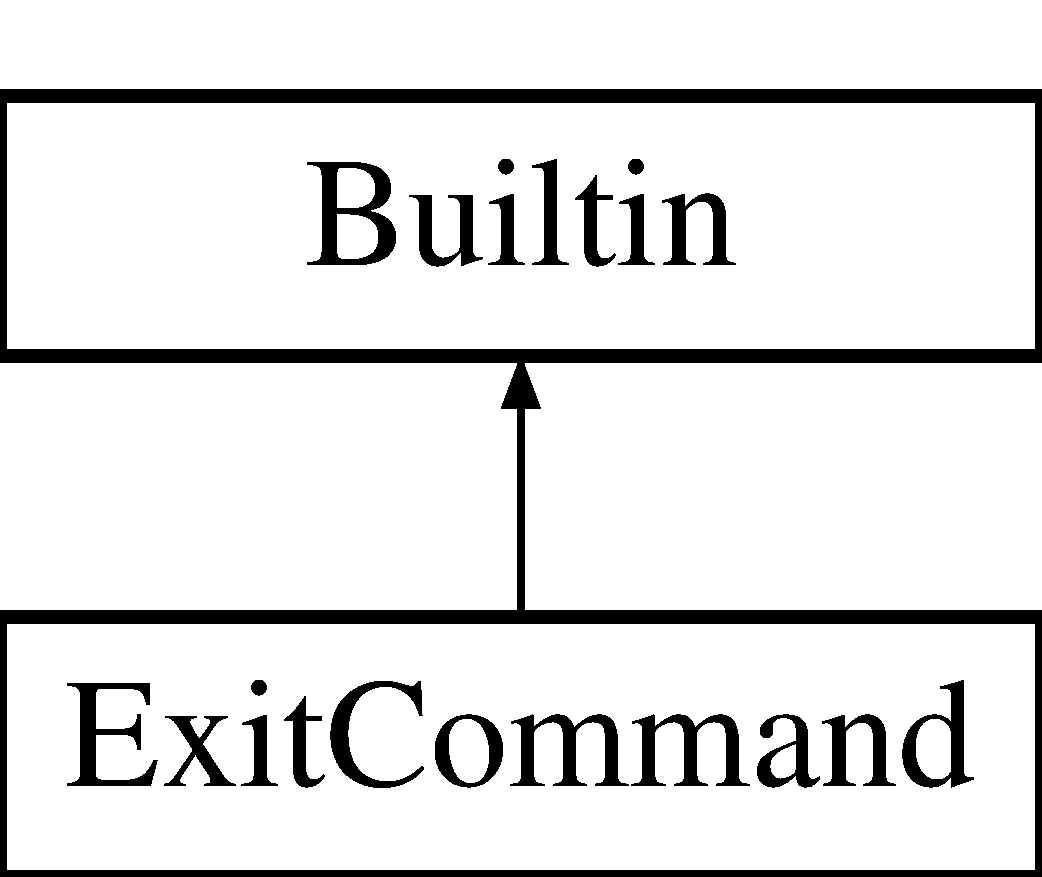
\includegraphics[height=2.000000cm]{classExitCommand}
\end{center}
\end{figure}


\subsection{Detailed Description}
Classe que implementa o comando exit. Sintaxe: exit, quit 

The documentation for this class was generated from the following files:\begin{DoxyCompactItemize}
\item 
\hyperlink{Builtin_8hpp}{Builtin.hpp}\item 
\hyperlink{Builtin_8cpp}{Builtin.cpp}\end{DoxyCompactItemize}

\hypertarget{classFgCommand}{
\section{FgCommand Class Reference}
\label{classFgCommand}\index{FgCommand@{FgCommand}}
}


{\ttfamily \#include $<$Builtin.hpp$>$}

Inheritance diagram for FgCommand:\begin{figure}[H]
\begin{center}
\leavevmode
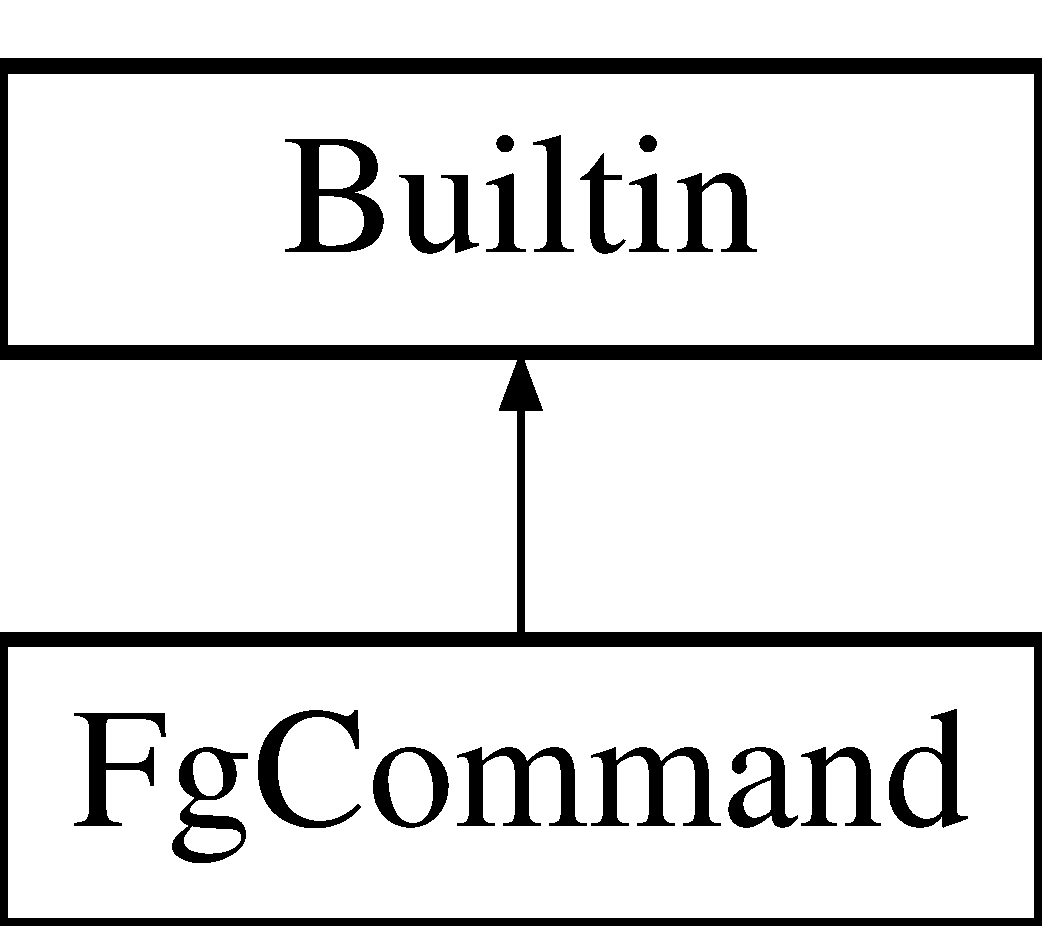
\includegraphics[height=2.000000cm]{classFgCommand}
\end{center}
\end{figure}


The documentation for this class was generated from the following files:\begin{DoxyCompactItemize}
\item 
\hyperlink{Builtin_8hpp}{Builtin.hpp}\item 
\hyperlink{Builtin_8cpp}{Builtin.cpp}\end{DoxyCompactItemize}

\hypertarget{structExecutor_1_1Job}{
\section{Executor::Job Struct Reference}
\label{structExecutor_1_1Job}\index{Executor::Job@{Executor::Job}}
}


Estrutura que representa um job. Guarda os dados necessarios para controlar processos.  




{\ttfamily \#include $<$Executor.hpp$>$}

\subsection*{Public Member Functions}
\begin{DoxyCompactItemize}
\item 
\hyperlink{structExecutor_1_1Job_aa6e1a092856e7ebc043adfb1eaa2c627}{Job} ()
\end{DoxyCompactItemize}
\subsection*{Public Attributes}
\begin{DoxyCompactItemize}
\item 
std::string \hyperlink{structExecutor_1_1Job_a38039efac2d62af668c99b63719f6125}{name}
\item 
pid\_\-t \hyperlink{structExecutor_1_1Job_a8d9163526e877fe1f603b66504ef8950}{pid}
\item 
unsigned \hyperlink{structExecutor_1_1Job_a9429fceffd304e1666ba1e8d0495c3f9}{jobid}
\item 
unsigned \hyperlink{structExecutor_1_1Job_ab3f85f9152e9b5457896f1b72fa8508c}{groupid}
\item 
bool \hyperlink{structExecutor_1_1Job_ac0ea0bc0c71fe4c1a2ad981df09fb5b0}{stopped}
\item 
bool \hyperlink{structExecutor_1_1Job_a7574b1ef35cd0dace06aee928fead108}{dead}
\end{DoxyCompactItemize}


\subsection{Detailed Description}
Estrutura que representa um job. Guarda os dados necessarios para controlar processos. \begin{DoxySeeAlso}{See also}
\hyperlink{classExecutor}{Executor} 
\end{DoxySeeAlso}


\subsection{Constructor \& Destructor Documentation}
\hypertarget{structExecutor_1_1Job_aa6e1a092856e7ebc043adfb1eaa2c627}{
\index{Executor::Job@{Executor::Job}!Job@{Job}}
\index{Job@{Job}!Executor::Job@{Executor::Job}}
\subsubsection[{Job}]{\setlength{\rightskip}{0pt plus 5cm}Executor::Job::Job (
\begin{DoxyParamCaption}
{}
\end{DoxyParamCaption}
)}}
\label{structExecutor_1_1Job_aa6e1a092856e7ebc043adfb1eaa2c627}


\subsection{Member Data Documentation}
\hypertarget{structExecutor_1_1Job_a7574b1ef35cd0dace06aee928fead108}{
\index{Executor::Job@{Executor::Job}!dead@{dead}}
\index{dead@{dead}!Executor::Job@{Executor::Job}}
\subsubsection[{dead}]{\setlength{\rightskip}{0pt plus 5cm}bool {\bf Executor::Job::dead}}}
\label{structExecutor_1_1Job_a7574b1ef35cd0dace06aee928fead108}
\hypertarget{structExecutor_1_1Job_ab3f85f9152e9b5457896f1b72fa8508c}{
\index{Executor::Job@{Executor::Job}!groupid@{groupid}}
\index{groupid@{groupid}!Executor::Job@{Executor::Job}}
\subsubsection[{groupid}]{\setlength{\rightskip}{0pt plus 5cm}unsigned {\bf Executor::Job::groupid}}}
\label{structExecutor_1_1Job_ab3f85f9152e9b5457896f1b72fa8508c}
\hypertarget{structExecutor_1_1Job_a9429fceffd304e1666ba1e8d0495c3f9}{
\index{Executor::Job@{Executor::Job}!jobid@{jobid}}
\index{jobid@{jobid}!Executor::Job@{Executor::Job}}
\subsubsection[{jobid}]{\setlength{\rightskip}{0pt plus 5cm}unsigned {\bf Executor::Job::jobid}}}
\label{structExecutor_1_1Job_a9429fceffd304e1666ba1e8d0495c3f9}
\hypertarget{structExecutor_1_1Job_a38039efac2d62af668c99b63719f6125}{
\index{Executor::Job@{Executor::Job}!name@{name}}
\index{name@{name}!Executor::Job@{Executor::Job}}
\subsubsection[{name}]{\setlength{\rightskip}{0pt plus 5cm}std::string {\bf Executor::Job::name}}}
\label{structExecutor_1_1Job_a38039efac2d62af668c99b63719f6125}
\hypertarget{structExecutor_1_1Job_a8d9163526e877fe1f603b66504ef8950}{
\index{Executor::Job@{Executor::Job}!pid@{pid}}
\index{pid@{pid}!Executor::Job@{Executor::Job}}
\subsubsection[{pid}]{\setlength{\rightskip}{0pt plus 5cm}pid\_\-t {\bf Executor::Job::pid}}}
\label{structExecutor_1_1Job_a8d9163526e877fe1f603b66504ef8950}
\hypertarget{structExecutor_1_1Job_ac0ea0bc0c71fe4c1a2ad981df09fb5b0}{
\index{Executor::Job@{Executor::Job}!stopped@{stopped}}
\index{stopped@{stopped}!Executor::Job@{Executor::Job}}
\subsubsection[{stopped}]{\setlength{\rightskip}{0pt plus 5cm}bool {\bf Executor::Job::stopped}}}
\label{structExecutor_1_1Job_ac0ea0bc0c71fe4c1a2ad981df09fb5b0}


The documentation for this struct was generated from the following files:\begin{DoxyCompactItemize}
\item 
\hyperlink{Executor_8hpp}{Executor.hpp}\item 
\hyperlink{Executor_8cpp}{Executor.cpp}\end{DoxyCompactItemize}

\hypertarget{classJobsCommand}{
\section{JobsCommand Class Reference}
\label{classJobsCommand}\index{JobsCommand@{JobsCommand}}
}


Classe que implementa o comando jobs.  




{\ttfamily \#include $<$Builtin.hpp$>$}

Inheritance diagram for JobsCommand:\begin{figure}[H]
\begin{center}
\leavevmode
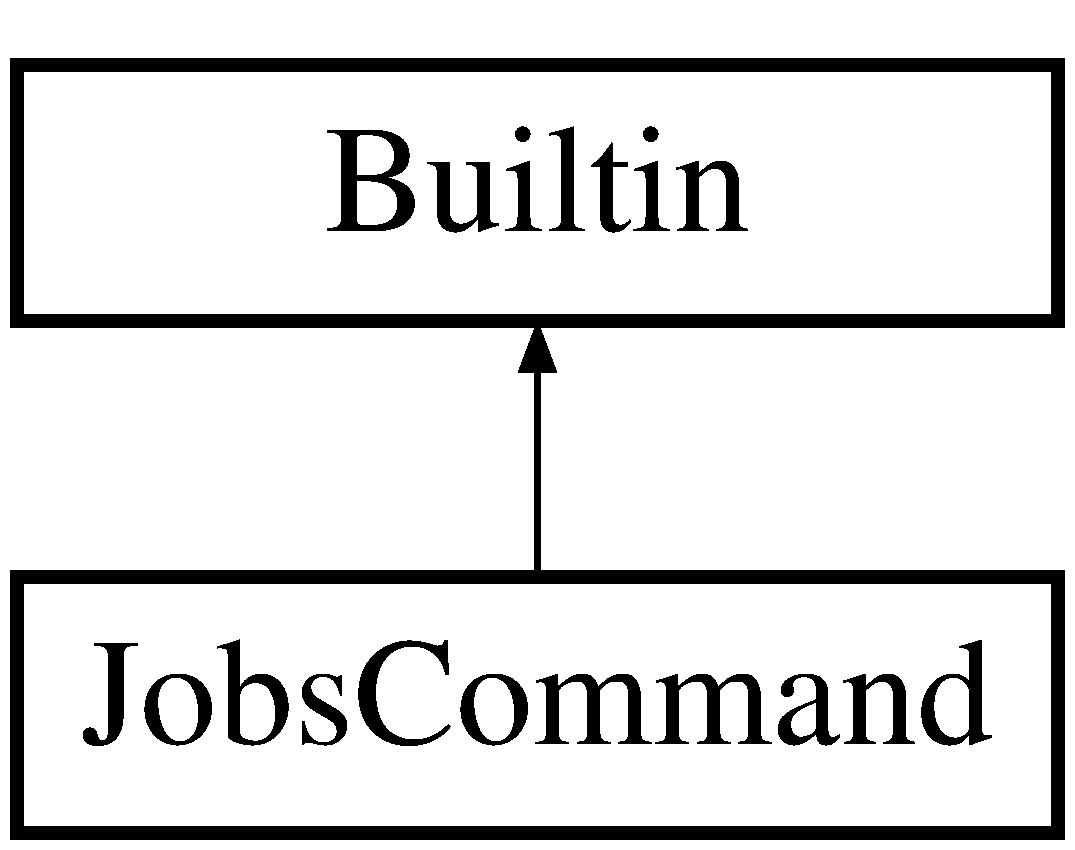
\includegraphics[height=2.000000cm]{classJobsCommand}
\end{center}
\end{figure}


\subsection{Detailed Description}
Classe que implementa o comando jobs. Sintaxe: jobs 

The documentation for this class was generated from the following files:\begin{DoxyCompactItemize}
\item 
\hyperlink{Builtin_8hpp}{Builtin.hpp}\item 
\hyperlink{Builtin_8cpp}{Builtin.cpp}\end{DoxyCompactItemize}

\hypertarget{classKillCommand}{
\section{KillCommand Class Reference}
\label{classKillCommand}\index{KillCommand@{KillCommand}}
}


Classe que implementa o comando kill.  




{\ttfamily \#include $<$Builtin.hpp$>$}

Inheritance diagram for KillCommand:\begin{figure}[H]
\begin{center}
\leavevmode
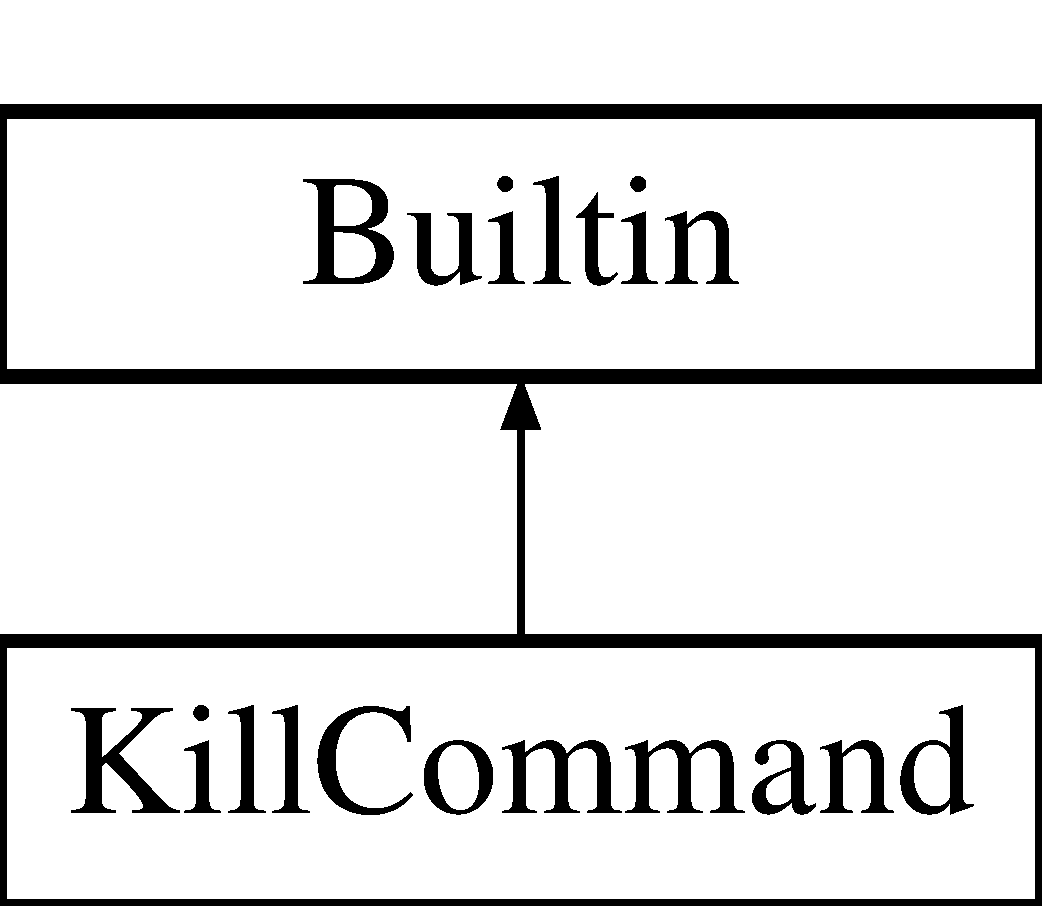
\includegraphics[height=2.000000cm]{classKillCommand}
\end{center}
\end{figure}


\subsection{Detailed Description}
Classe que implementa o comando kill. Sintaxe: kill \%$<$JOBID$>$ 

The documentation for this class was generated from the following files:\begin{DoxyCompactItemize}
\item 
\hyperlink{Builtin_8hpp}{Builtin.hpp}\item 
\hyperlink{Builtin_8cpp}{Builtin.cpp}\end{DoxyCompactItemize}

\hypertarget{classMyTypo}{
\section{MyTypo Class Reference}
\label{classMyTypo}\index{MyTypo@{MyTypo}}
}


Firulas.  




{\ttfamily \#include $<$MyTypo.hpp$>$}

\subsection*{Public Types}
\begin{DoxyCompactItemize}
\item 
enum \hyperlink{classMyTypo_a8def2c649b389845fc9ef0425d6ba3f3}{Style} \{ \par
\hyperlink{classMyTypo_a8def2c649b389845fc9ef0425d6ba3f3a77b0bcc2d2ad397aaf217b9925311286}{NORMAL} =  0, 
\hyperlink{classMyTypo_a8def2c649b389845fc9ef0425d6ba3f3a7b77c3671053b7cecb4f5f62d5f3dacd}{BOLD}, 
\hyperlink{classMyTypo_a8def2c649b389845fc9ef0425d6ba3f3a092275401d9e91f117091f7f830c4537}{UNDER} =  4, 
\hyperlink{classMyTypo_a8def2c649b389845fc9ef0425d6ba3f3aeba436648705fd91802eca94dd774bef}{BLINK}, 
\par
\hyperlink{classMyTypo_a8def2c649b389845fc9ef0425d6ba3f3a072b22b51d23b6ba5507658851b1508a}{INVERT} =  7
 \}
\item 
enum \hyperlink{classMyTypo_a82023ae74e9c64ec7b6e57d54df708ea}{Foreground} \{ \par
\hyperlink{classMyTypo_a82023ae74e9c64ec7b6e57d54df708eaa5d485cc852fd8925db5f58724949ed7d}{BLACK} =  30, 
\hyperlink{classMyTypo_a82023ae74e9c64ec7b6e57d54df708eaae9a6714a38c1570a628c92d992b8886a}{RED}, 
\hyperlink{classMyTypo_a82023ae74e9c64ec7b6e57d54df708eaac0090bdb54450325945e1eec5f3240df}{GREEN}, 
\hyperlink{classMyTypo_a82023ae74e9c64ec7b6e57d54df708eaa3980d41699961553b6365178968e1235}{BROWN}, 
\par
\hyperlink{classMyTypo_a82023ae74e9c64ec7b6e57d54df708eaae3d9ddbcc3cceb11912943b7647b3842}{BLUE}, 
\hyperlink{classMyTypo_a82023ae74e9c64ec7b6e57d54df708eaa49a268a91b8ed1b28ea8518bed685029}{PURPLE}, 
\hyperlink{classMyTypo_a82023ae74e9c64ec7b6e57d54df708eaa20a754710244898038b406234e73682e}{CYAN}, 
\hyperlink{classMyTypo_a82023ae74e9c64ec7b6e57d54df708eaaa48d0f298f2b7be62cd7dc84d6b7a999}{GRAY}
 \}
\item 
enum \hyperlink{classMyTypo_ac6643b465e94f6ecb7fb650c4b3531e8}{Background} \{ \par
\hyperlink{classMyTypo_ac6643b465e94f6ecb7fb650c4b3531e8ab5db6d6b3a486ef6d773c3c04c1281b4}{B\_\-TRANSPARENT} =  -\/1, 
\hyperlink{classMyTypo_ac6643b465e94f6ecb7fb650c4b3531e8ac2e0d75a46d7044e594d4f89cb76b4ca}{B\_\-BLACK} =  40, 
\hyperlink{classMyTypo_ac6643b465e94f6ecb7fb650c4b3531e8aeb1941bfc2f16a35302f10000684a6ef}{B\_\-RED}, 
\hyperlink{classMyTypo_ac6643b465e94f6ecb7fb650c4b3531e8aac6076a603ab6c8be9a700e115c01453}{B\_\-GREEN}, 
\par
\hyperlink{classMyTypo_ac6643b465e94f6ecb7fb650c4b3531e8afd8a2faa10bc6f4f68066e8a8064ec3f}{B\_\-BROWN}, 
\hyperlink{classMyTypo_ac6643b465e94f6ecb7fb650c4b3531e8a08b6e71d66570f7a3e34cc7995e85317}{B\_\-BLUE}, 
\hyperlink{classMyTypo_ac6643b465e94f6ecb7fb650c4b3531e8a4d7b53c84bb3c21ca6adae139dca95de}{B\_\-PURPLE}, 
\hyperlink{classMyTypo_ac6643b465e94f6ecb7fb650c4b3531e8a6762080d090818122cabaf479be290a6}{B\_\-CYAN}, 
\par
\hyperlink{classMyTypo_ac6643b465e94f6ecb7fb650c4b3531e8a85f06fb2e3d8b757294edc6eecabf43e}{B\_\-GRAY}
 \}
\end{DoxyCompactItemize}
\subsection*{Public Member Functions}
\begin{DoxyCompactItemize}
\item 
void \hyperlink{classMyTypo_a3422166dfc3911a36c32271e0434587d}{set\_\-foreground} (int color)
\item 
void \hyperlink{classMyTypo_a325589499eb8e5c4b52355011f7b9cf3}{set\_\-background} (int color)
\item 
void \hyperlink{classMyTypo_a94dc39fef3ca57dc956deda92514c648}{set\_\-style} (int color)
\item 
int \hyperlink{classMyTypo_a554372a4548dda7c157d69fe0651a23f}{get\_\-foreground} (void)
\item 
int \hyperlink{classMyTypo_ad935060c132f772a2a1239bc6426d5de}{get\_\-background} (void)
\item 
int \hyperlink{classMyTypo_af181779fdfb0eb793136408e2a4fec94}{get\_\-style} (void)
\item 
bool \hyperlink{classMyTypo_ad44b40659d3e5cf17f22677264ca6ab9}{get\_\-opened} (void)
\item 
\hyperlink{classMyTypo_a7ab56324aa7eb1bf6efca62d14d07bee}{MyTypo} (int style=NORMAL, int foreground=BLACK, int background=B\_\-TRANSPARENT)
\item 
void \hyperlink{classMyTypo_ac0cf15a492908e3efdc6b57e1eff4390}{toogleOpened} (void)
\item 
void \hyperlink{classMyTypo_ab1f48a8f65a17b5240c393af75ef2657}{setParameters} (int style=NORMAL, int foreground=BLACK, int background=B\_\-TRANSPARENT)
\item 
std::ostream \& \hyperlink{classMyTypo_ae352299f62ef344e98f10a900546c83c}{openTag} (std::ostream \&ost)
\item 
std::ostream \& \hyperlink{classMyTypo_a6572b9b25e66990a26308e6bbc9ec301}{closeTag} (std::ostream \&ost)
\end{DoxyCompactItemize}


\subsection{Detailed Description}
Firulas. Serve apenas para deixar a saida mais bonita, com diferentes cores e estilos para a fonte, no terminal 

\subsection{Member Enumeration Documentation}
\hypertarget{classMyTypo_ac6643b465e94f6ecb7fb650c4b3531e8}{
\index{MyTypo@{MyTypo}!Background@{Background}}
\index{Background@{Background}!MyTypo@{MyTypo}}
\subsubsection[{Background}]{\setlength{\rightskip}{0pt plus 5cm}enum {\bf MyTypo::Background}}}
\label{classMyTypo_ac6643b465e94f6ecb7fb650c4b3531e8}
\begin{Desc}
\item[Enumerator: ]\par
\begin{description}
\index{B\_\-TRANSPARENT@{B\_\-TRANSPARENT}!MyTypo@{MyTypo}}\index{MyTypo@{MyTypo}!B\_\-TRANSPARENT@{B\_\-TRANSPARENT}}\item[{\em 
\hypertarget{classMyTypo_ac6643b465e94f6ecb7fb650c4b3531e8ab5db6d6b3a486ef6d773c3c04c1281b4}{
B\_\-TRANSPARENT}
\label{classMyTypo_ac6643b465e94f6ecb7fb650c4b3531e8ab5db6d6b3a486ef6d773c3c04c1281b4}
}]\index{B\_\-BLACK@{B\_\-BLACK}!MyTypo@{MyTypo}}\index{MyTypo@{MyTypo}!B\_\-BLACK@{B\_\-BLACK}}\item[{\em 
\hypertarget{classMyTypo_ac6643b465e94f6ecb7fb650c4b3531e8ac2e0d75a46d7044e594d4f89cb76b4ca}{
B\_\-BLACK}
\label{classMyTypo_ac6643b465e94f6ecb7fb650c4b3531e8ac2e0d75a46d7044e594d4f89cb76b4ca}
}]\index{B\_\-RED@{B\_\-RED}!MyTypo@{MyTypo}}\index{MyTypo@{MyTypo}!B\_\-RED@{B\_\-RED}}\item[{\em 
\hypertarget{classMyTypo_ac6643b465e94f6ecb7fb650c4b3531e8aeb1941bfc2f16a35302f10000684a6ef}{
B\_\-RED}
\label{classMyTypo_ac6643b465e94f6ecb7fb650c4b3531e8aeb1941bfc2f16a35302f10000684a6ef}
}]\index{B\_\-GREEN@{B\_\-GREEN}!MyTypo@{MyTypo}}\index{MyTypo@{MyTypo}!B\_\-GREEN@{B\_\-GREEN}}\item[{\em 
\hypertarget{classMyTypo_ac6643b465e94f6ecb7fb650c4b3531e8aac6076a603ab6c8be9a700e115c01453}{
B\_\-GREEN}
\label{classMyTypo_ac6643b465e94f6ecb7fb650c4b3531e8aac6076a603ab6c8be9a700e115c01453}
}]\index{B\_\-BROWN@{B\_\-BROWN}!MyTypo@{MyTypo}}\index{MyTypo@{MyTypo}!B\_\-BROWN@{B\_\-BROWN}}\item[{\em 
\hypertarget{classMyTypo_ac6643b465e94f6ecb7fb650c4b3531e8afd8a2faa10bc6f4f68066e8a8064ec3f}{
B\_\-BROWN}
\label{classMyTypo_ac6643b465e94f6ecb7fb650c4b3531e8afd8a2faa10bc6f4f68066e8a8064ec3f}
}]\index{B\_\-BLUE@{B\_\-BLUE}!MyTypo@{MyTypo}}\index{MyTypo@{MyTypo}!B\_\-BLUE@{B\_\-BLUE}}\item[{\em 
\hypertarget{classMyTypo_ac6643b465e94f6ecb7fb650c4b3531e8a08b6e71d66570f7a3e34cc7995e85317}{
B\_\-BLUE}
\label{classMyTypo_ac6643b465e94f6ecb7fb650c4b3531e8a08b6e71d66570f7a3e34cc7995e85317}
}]\index{B\_\-PURPLE@{B\_\-PURPLE}!MyTypo@{MyTypo}}\index{MyTypo@{MyTypo}!B\_\-PURPLE@{B\_\-PURPLE}}\item[{\em 
\hypertarget{classMyTypo_ac6643b465e94f6ecb7fb650c4b3531e8a4d7b53c84bb3c21ca6adae139dca95de}{
B\_\-PURPLE}
\label{classMyTypo_ac6643b465e94f6ecb7fb650c4b3531e8a4d7b53c84bb3c21ca6adae139dca95de}
}]\index{B\_\-CYAN@{B\_\-CYAN}!MyTypo@{MyTypo}}\index{MyTypo@{MyTypo}!B\_\-CYAN@{B\_\-CYAN}}\item[{\em 
\hypertarget{classMyTypo_ac6643b465e94f6ecb7fb650c4b3531e8a6762080d090818122cabaf479be290a6}{
B\_\-CYAN}
\label{classMyTypo_ac6643b465e94f6ecb7fb650c4b3531e8a6762080d090818122cabaf479be290a6}
}]\index{B\_\-GRAY@{B\_\-GRAY}!MyTypo@{MyTypo}}\index{MyTypo@{MyTypo}!B\_\-GRAY@{B\_\-GRAY}}\item[{\em 
\hypertarget{classMyTypo_ac6643b465e94f6ecb7fb650c4b3531e8a85f06fb2e3d8b757294edc6eecabf43e}{
B\_\-GRAY}
\label{classMyTypo_ac6643b465e94f6ecb7fb650c4b3531e8a85f06fb2e3d8b757294edc6eecabf43e}
}]\end{description}
\end{Desc}

\hypertarget{classMyTypo_a82023ae74e9c64ec7b6e57d54df708ea}{
\index{MyTypo@{MyTypo}!Foreground@{Foreground}}
\index{Foreground@{Foreground}!MyTypo@{MyTypo}}
\subsubsection[{Foreground}]{\setlength{\rightskip}{0pt plus 5cm}enum {\bf MyTypo::Foreground}}}
\label{classMyTypo_a82023ae74e9c64ec7b6e57d54df708ea}
\begin{Desc}
\item[Enumerator: ]\par
\begin{description}
\index{BLACK@{BLACK}!MyTypo@{MyTypo}}\index{MyTypo@{MyTypo}!BLACK@{BLACK}}\item[{\em 
\hypertarget{classMyTypo_a82023ae74e9c64ec7b6e57d54df708eaa5d485cc852fd8925db5f58724949ed7d}{
BLACK}
\label{classMyTypo_a82023ae74e9c64ec7b6e57d54df708eaa5d485cc852fd8925db5f58724949ed7d}
}]\index{RED@{RED}!MyTypo@{MyTypo}}\index{MyTypo@{MyTypo}!RED@{RED}}\item[{\em 
\hypertarget{classMyTypo_a82023ae74e9c64ec7b6e57d54df708eaae9a6714a38c1570a628c92d992b8886a}{
RED}
\label{classMyTypo_a82023ae74e9c64ec7b6e57d54df708eaae9a6714a38c1570a628c92d992b8886a}
}]\index{GREEN@{GREEN}!MyTypo@{MyTypo}}\index{MyTypo@{MyTypo}!GREEN@{GREEN}}\item[{\em 
\hypertarget{classMyTypo_a82023ae74e9c64ec7b6e57d54df708eaac0090bdb54450325945e1eec5f3240df}{
GREEN}
\label{classMyTypo_a82023ae74e9c64ec7b6e57d54df708eaac0090bdb54450325945e1eec5f3240df}
}]\index{BROWN@{BROWN}!MyTypo@{MyTypo}}\index{MyTypo@{MyTypo}!BROWN@{BROWN}}\item[{\em 
\hypertarget{classMyTypo_a82023ae74e9c64ec7b6e57d54df708eaa3980d41699961553b6365178968e1235}{
BROWN}
\label{classMyTypo_a82023ae74e9c64ec7b6e57d54df708eaa3980d41699961553b6365178968e1235}
}]\index{BLUE@{BLUE}!MyTypo@{MyTypo}}\index{MyTypo@{MyTypo}!BLUE@{BLUE}}\item[{\em 
\hypertarget{classMyTypo_a82023ae74e9c64ec7b6e57d54df708eaae3d9ddbcc3cceb11912943b7647b3842}{
BLUE}
\label{classMyTypo_a82023ae74e9c64ec7b6e57d54df708eaae3d9ddbcc3cceb11912943b7647b3842}
}]\index{PURPLE@{PURPLE}!MyTypo@{MyTypo}}\index{MyTypo@{MyTypo}!PURPLE@{PURPLE}}\item[{\em 
\hypertarget{classMyTypo_a82023ae74e9c64ec7b6e57d54df708eaa49a268a91b8ed1b28ea8518bed685029}{
PURPLE}
\label{classMyTypo_a82023ae74e9c64ec7b6e57d54df708eaa49a268a91b8ed1b28ea8518bed685029}
}]\index{CYAN@{CYAN}!MyTypo@{MyTypo}}\index{MyTypo@{MyTypo}!CYAN@{CYAN}}\item[{\em 
\hypertarget{classMyTypo_a82023ae74e9c64ec7b6e57d54df708eaa20a754710244898038b406234e73682e}{
CYAN}
\label{classMyTypo_a82023ae74e9c64ec7b6e57d54df708eaa20a754710244898038b406234e73682e}
}]\index{GRAY@{GRAY}!MyTypo@{MyTypo}}\index{MyTypo@{MyTypo}!GRAY@{GRAY}}\item[{\em 
\hypertarget{classMyTypo_a82023ae74e9c64ec7b6e57d54df708eaaa48d0f298f2b7be62cd7dc84d6b7a999}{
GRAY}
\label{classMyTypo_a82023ae74e9c64ec7b6e57d54df708eaaa48d0f298f2b7be62cd7dc84d6b7a999}
}]\end{description}
\end{Desc}

\hypertarget{classMyTypo_a8def2c649b389845fc9ef0425d6ba3f3}{
\index{MyTypo@{MyTypo}!Style@{Style}}
\index{Style@{Style}!MyTypo@{MyTypo}}
\subsubsection[{Style}]{\setlength{\rightskip}{0pt plus 5cm}enum {\bf MyTypo::Style}}}
\label{classMyTypo_a8def2c649b389845fc9ef0425d6ba3f3}
\begin{Desc}
\item[Enumerator: ]\par
\begin{description}
\index{NORMAL@{NORMAL}!MyTypo@{MyTypo}}\index{MyTypo@{MyTypo}!NORMAL@{NORMAL}}\item[{\em 
\hypertarget{classMyTypo_a8def2c649b389845fc9ef0425d6ba3f3a77b0bcc2d2ad397aaf217b9925311286}{
NORMAL}
\label{classMyTypo_a8def2c649b389845fc9ef0425d6ba3f3a77b0bcc2d2ad397aaf217b9925311286}
}]\index{BOLD@{BOLD}!MyTypo@{MyTypo}}\index{MyTypo@{MyTypo}!BOLD@{BOLD}}\item[{\em 
\hypertarget{classMyTypo_a8def2c649b389845fc9ef0425d6ba3f3a7b77c3671053b7cecb4f5f62d5f3dacd}{
BOLD}
\label{classMyTypo_a8def2c649b389845fc9ef0425d6ba3f3a7b77c3671053b7cecb4f5f62d5f3dacd}
}]\index{UNDER@{UNDER}!MyTypo@{MyTypo}}\index{MyTypo@{MyTypo}!UNDER@{UNDER}}\item[{\em 
\hypertarget{classMyTypo_a8def2c649b389845fc9ef0425d6ba3f3a092275401d9e91f117091f7f830c4537}{
UNDER}
\label{classMyTypo_a8def2c649b389845fc9ef0425d6ba3f3a092275401d9e91f117091f7f830c4537}
}]\index{BLINK@{BLINK}!MyTypo@{MyTypo}}\index{MyTypo@{MyTypo}!BLINK@{BLINK}}\item[{\em 
\hypertarget{classMyTypo_a8def2c649b389845fc9ef0425d6ba3f3aeba436648705fd91802eca94dd774bef}{
BLINK}
\label{classMyTypo_a8def2c649b389845fc9ef0425d6ba3f3aeba436648705fd91802eca94dd774bef}
}]\index{INVERT@{INVERT}!MyTypo@{MyTypo}}\index{MyTypo@{MyTypo}!INVERT@{INVERT}}\item[{\em 
\hypertarget{classMyTypo_a8def2c649b389845fc9ef0425d6ba3f3a072b22b51d23b6ba5507658851b1508a}{
INVERT}
\label{classMyTypo_a8def2c649b389845fc9ef0425d6ba3f3a072b22b51d23b6ba5507658851b1508a}
}]\end{description}
\end{Desc}



\subsection{Constructor \& Destructor Documentation}
\hypertarget{classMyTypo_a7ab56324aa7eb1bf6efca62d14d07bee}{
\index{MyTypo@{MyTypo}!MyTypo@{MyTypo}}
\index{MyTypo@{MyTypo}!MyTypo@{MyTypo}}
\subsubsection[{MyTypo}]{\setlength{\rightskip}{0pt plus 5cm}MyTypo::MyTypo (
\begin{DoxyParamCaption}
\item[{int}]{style = {\ttfamily NORMAL}, }
\item[{int}]{foreground = {\ttfamily BLACK}, }
\item[{int}]{background = {\ttfamily B\_\-TRANSPARENT}}
\end{DoxyParamCaption}
)}}
\label{classMyTypo_a7ab56324aa7eb1bf6efca62d14d07bee}


\subsection{Member Function Documentation}
\hypertarget{classMyTypo_a6572b9b25e66990a26308e6bbc9ec301}{
\index{MyTypo@{MyTypo}!closeTag@{closeTag}}
\index{closeTag@{closeTag}!MyTypo@{MyTypo}}
\subsubsection[{closeTag}]{\setlength{\rightskip}{0pt plus 5cm}std::ostream \& MyTypo::closeTag (
\begin{DoxyParamCaption}
\item[{std::ostream \&}]{ost}
\end{DoxyParamCaption}
)}}
\label{classMyTypo_a6572b9b25e66990a26308e6bbc9ec301}
\hypertarget{classMyTypo_ad935060c132f772a2a1239bc6426d5de}{
\index{MyTypo@{MyTypo}!get\_\-background@{get\_\-background}}
\index{get\_\-background@{get\_\-background}!MyTypo@{MyTypo}}
\subsubsection[{get\_\-background}]{\setlength{\rightskip}{0pt plus 5cm}int MyTypo::get\_\-background (
\begin{DoxyParamCaption}
\item[{void}]{}
\end{DoxyParamCaption}
)}}
\label{classMyTypo_ad935060c132f772a2a1239bc6426d5de}
\hypertarget{classMyTypo_a554372a4548dda7c157d69fe0651a23f}{
\index{MyTypo@{MyTypo}!get\_\-foreground@{get\_\-foreground}}
\index{get\_\-foreground@{get\_\-foreground}!MyTypo@{MyTypo}}
\subsubsection[{get\_\-foreground}]{\setlength{\rightskip}{0pt plus 5cm}int MyTypo::get\_\-foreground (
\begin{DoxyParamCaption}
\item[{void}]{}
\end{DoxyParamCaption}
)}}
\label{classMyTypo_a554372a4548dda7c157d69fe0651a23f}
\hypertarget{classMyTypo_ad44b40659d3e5cf17f22677264ca6ab9}{
\index{MyTypo@{MyTypo}!get\_\-opened@{get\_\-opened}}
\index{get\_\-opened@{get\_\-opened}!MyTypo@{MyTypo}}
\subsubsection[{get\_\-opened}]{\setlength{\rightskip}{0pt plus 5cm}bool MyTypo::get\_\-opened (
\begin{DoxyParamCaption}
\item[{void}]{}
\end{DoxyParamCaption}
)}}
\label{classMyTypo_ad44b40659d3e5cf17f22677264ca6ab9}
\hypertarget{classMyTypo_af181779fdfb0eb793136408e2a4fec94}{
\index{MyTypo@{MyTypo}!get\_\-style@{get\_\-style}}
\index{get\_\-style@{get\_\-style}!MyTypo@{MyTypo}}
\subsubsection[{get\_\-style}]{\setlength{\rightskip}{0pt plus 5cm}int MyTypo::get\_\-style (
\begin{DoxyParamCaption}
\item[{void}]{}
\end{DoxyParamCaption}
)}}
\label{classMyTypo_af181779fdfb0eb793136408e2a4fec94}
\hypertarget{classMyTypo_ae352299f62ef344e98f10a900546c83c}{
\index{MyTypo@{MyTypo}!openTag@{openTag}}
\index{openTag@{openTag}!MyTypo@{MyTypo}}
\subsubsection[{openTag}]{\setlength{\rightskip}{0pt plus 5cm}std::ostream \& MyTypo::openTag (
\begin{DoxyParamCaption}
\item[{std::ostream \&}]{ost}
\end{DoxyParamCaption}
)}}
\label{classMyTypo_ae352299f62ef344e98f10a900546c83c}
\hypertarget{classMyTypo_a325589499eb8e5c4b52355011f7b9cf3}{
\index{MyTypo@{MyTypo}!set\_\-background@{set\_\-background}}
\index{set\_\-background@{set\_\-background}!MyTypo@{MyTypo}}
\subsubsection[{set\_\-background}]{\setlength{\rightskip}{0pt plus 5cm}void MyTypo::set\_\-background (
\begin{DoxyParamCaption}
\item[{int}]{color}
\end{DoxyParamCaption}
)}}
\label{classMyTypo_a325589499eb8e5c4b52355011f7b9cf3}
\hypertarget{classMyTypo_a3422166dfc3911a36c32271e0434587d}{
\index{MyTypo@{MyTypo}!set\_\-foreground@{set\_\-foreground}}
\index{set\_\-foreground@{set\_\-foreground}!MyTypo@{MyTypo}}
\subsubsection[{set\_\-foreground}]{\setlength{\rightskip}{0pt plus 5cm}void MyTypo::set\_\-foreground (
\begin{DoxyParamCaption}
\item[{int}]{color}
\end{DoxyParamCaption}
)}}
\label{classMyTypo_a3422166dfc3911a36c32271e0434587d}
\hypertarget{classMyTypo_a94dc39fef3ca57dc956deda92514c648}{
\index{MyTypo@{MyTypo}!set\_\-style@{set\_\-style}}
\index{set\_\-style@{set\_\-style}!MyTypo@{MyTypo}}
\subsubsection[{set\_\-style}]{\setlength{\rightskip}{0pt plus 5cm}void MyTypo::set\_\-style (
\begin{DoxyParamCaption}
\item[{int}]{color}
\end{DoxyParamCaption}
)}}
\label{classMyTypo_a94dc39fef3ca57dc956deda92514c648}
\hypertarget{classMyTypo_ab1f48a8f65a17b5240c393af75ef2657}{
\index{MyTypo@{MyTypo}!setParameters@{setParameters}}
\index{setParameters@{setParameters}!MyTypo@{MyTypo}}
\subsubsection[{setParameters}]{\setlength{\rightskip}{0pt plus 5cm}void MyTypo::setParameters (
\begin{DoxyParamCaption}
\item[{int}]{style = {\ttfamily NORMAL}, }
\item[{int}]{foreground = {\ttfamily BLACK}, }
\item[{int}]{background = {\ttfamily B\_\-TRANSPARENT}}
\end{DoxyParamCaption}
)}}
\label{classMyTypo_ab1f48a8f65a17b5240c393af75ef2657}
\hypertarget{classMyTypo_ac0cf15a492908e3efdc6b57e1eff4390}{
\index{MyTypo@{MyTypo}!toogleOpened@{toogleOpened}}
\index{toogleOpened@{toogleOpened}!MyTypo@{MyTypo}}
\subsubsection[{toogleOpened}]{\setlength{\rightskip}{0pt plus 5cm}void MyTypo::toogleOpened (
\begin{DoxyParamCaption}
\item[{void}]{}
\end{DoxyParamCaption}
)}}
\label{classMyTypo_ac0cf15a492908e3efdc6b57e1eff4390}


The documentation for this class was generated from the following files:\begin{DoxyCompactItemize}
\item 
\hyperlink{MyTypo_8hpp}{MyTypo.hpp}\item 
\hyperlink{MyTypo_8cpp}{MyTypo.cpp}\end{DoxyCompactItemize}

\hypertarget{classParser}{
\section{Parser Class Reference}
\label{classParser}\index{Parser@{Parser}}
}


Utilizado para converter a entrada do usuario em uma \hyperlink{classCommandLine}{CommandLine}.  




{\ttfamily \#include $<$Parser.hpp$>$}

\subsection*{Public Member Functions}
\begin{DoxyCompactItemize}
\item 
\hyperlink{classParser_a12234f6cd36b61af4b50c94a179422c1}{Parser} ()
\item 
\hyperlink{classCommandLine}{CommandLine} $\ast$ \hyperlink{classParser_a992f6612be5ab4a587e29c7ed5c824c3}{readCommandLine} ()
\item 
bool \hyperlink{classParser_a2d6e80902c93ceed3d8f9a2f7cacd50c}{newLine} ()
\end{DoxyCompactItemize}


\subsection{Detailed Description}
Utilizado para converter a entrada do usuario em uma \hyperlink{classCommandLine}{CommandLine}. A linha de usuario deve ter a seguinte forma\par
 $<$comando$>$$<$paramentro$>$...$<$parametro$>$$|$...$|$$<$comando$>$...\mbox{[}$<$ $<$entrada$>$\mbox{]}\mbox{[}\mbox{[}1$>$$|$$>$$|$$>$$>$\mbox{]}\mbox{[}2$>$\mbox{]}$<$saida$>$$|$\&$>$$<$saida$>$\mbox{]}\mbox{[}\&\mbox{]} 

\subsection{Constructor \& Destructor Documentation}
\hypertarget{classParser_a12234f6cd36b61af4b50c94a179422c1}{
\index{Parser@{Parser}!Parser@{Parser}}
\index{Parser@{Parser}!Parser@{Parser}}
\subsubsection[{Parser}]{\setlength{\rightskip}{0pt plus 5cm}Parser::Parser (
\begin{DoxyParamCaption}
{}
\end{DoxyParamCaption}
)}}
\label{classParser_a12234f6cd36b61af4b50c94a179422c1}


\subsection{Member Function Documentation}
\hypertarget{classParser_a2d6e80902c93ceed3d8f9a2f7cacd50c}{
\index{Parser@{Parser}!newLine@{newLine}}
\index{newLine@{newLine}!Parser@{Parser}}
\subsubsection[{newLine}]{\setlength{\rightskip}{0pt plus 5cm}bool Parser::newLine (
\begin{DoxyParamCaption}
{}
\end{DoxyParamCaption}
)}}
\label{classParser_a2d6e80902c93ceed3d8f9a2f7cacd50c}
\begin{DoxyReturn}{Returns}
Verdadeiro caso esteja em uma nova linha de comando (nao necessariamente endl, mas fim da pipeline por \& 
\end{DoxyReturn}
\hypertarget{classParser_a992f6612be5ab4a587e29c7ed5c824c3}{
\index{Parser@{Parser}!readCommandLine@{readCommandLine}}
\index{readCommandLine@{readCommandLine}!Parser@{Parser}}
\subsubsection[{readCommandLine}]{\setlength{\rightskip}{0pt plus 5cm}{\bf CommandLine} $\ast$ Parser::readCommandLine (
\begin{DoxyParamCaption}
{}
\end{DoxyParamCaption}
)}}
\label{classParser_a992f6612be5ab4a587e29c7ed5c824c3}
\begin{DoxyReturn}{Returns}
Le e interpreta uma linha de comando dada pelo usuario no stdin 
\end{DoxyReturn}


The documentation for this class was generated from the following files:\begin{DoxyCompactItemize}
\item 
\hyperlink{Parser_8hpp}{Parser.hpp}\item 
\hyperlink{Parser_8cpp}{Parser.cpp}\end{DoxyCompactItemize}

\hypertarget{classProgram}{
\section{Program Class Reference}
\label{classProgram}\index{Program@{Program}}
}


{\ttfamily \#include $<$Program.hpp$>$}

\subsection*{Public Member Functions}
\begin{DoxyCompactItemize}
\item 
int \hyperlink{classProgram_ab7cb58a80ead351385709a33c4491db1}{run} ()
\end{DoxyCompactItemize}


\subsection{Member Function Documentation}
\hypertarget{classProgram_ab7cb58a80ead351385709a33c4491db1}{
\index{Program@{Program}!run@{run}}
\index{run@{run}!Program@{Program}}
\subsubsection[{run}]{\setlength{\rightskip}{0pt plus 5cm}int Program::run (
\begin{DoxyParamCaption}
{}
\end{DoxyParamCaption}
)}}
\label{classProgram_ab7cb58a80ead351385709a33c4491db1}


The documentation for this class was generated from the following files:\begin{DoxyCompactItemize}
\item 
\hyperlink{Program_8hpp}{Program.hpp}\item 
\hyperlink{Program_8cpp}{Program.cpp}\end{DoxyCompactItemize}

\hypertarget{classPwdCommand}{
\section{PwdCommand Class Reference}
\label{classPwdCommand}\index{PwdCommand@{PwdCommand}}
}


Classe que implementa o comando pwd. Sintaxe: pwd.  




{\ttfamily \#include $<$Builtin.hpp$>$}

Inheritance diagram for PwdCommand:\begin{figure}[H]
\begin{center}
\leavevmode
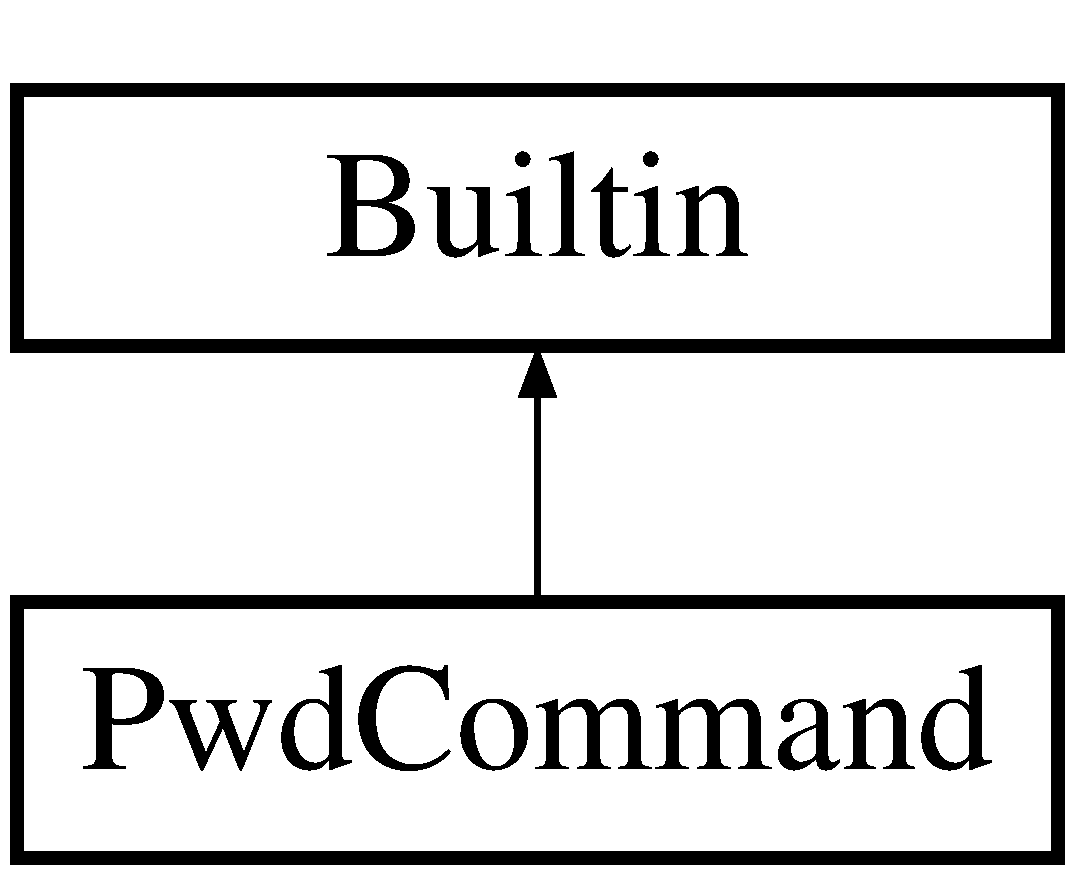
\includegraphics[height=2.000000cm]{classPwdCommand}
\end{center}
\end{figure}


\subsection{Detailed Description}
Classe que implementa o comando pwd. Sintaxe: pwd. 

The documentation for this class was generated from the following files:\begin{DoxyCompactItemize}
\item 
\hyperlink{Builtin_8hpp}{Builtin.hpp}\item 
\hyperlink{Builtin_8cpp}{Builtin.cpp}\end{DoxyCompactItemize}

\chapter{File Documentation}
\hypertarget{Builtin_8cpp}{
\section{Builtin.cpp File Reference}
\label{Builtin_8cpp}\index{Builtin.cpp@{Builtin.cpp}}
}
{\ttfamily \#include \char`\"{}Builtin.hpp\char`\"{}}\par
{\ttfamily \#include $<$unistd.h$>$}\par
{\ttfamily \#include $<$iostream$>$}\par
{\ttfamily \#include $<$list$>$}\par
{\ttfamily \#include \char`\"{}MyTypo.hpp\char`\"{}}\par
{\ttfamily \#include $<$cstdio$>$}\par
{\ttfamily \#include $<$cstdlib$>$}\par
{\ttfamily \#include $<$signal.h$>$}\par
{\ttfamily \#include $<$sys/types.h$>$}\par
{\ttfamily \#include $<$sys/wait.h$>$}\par
{\ttfamily \#include \char`\"{}Handlers.hpp\char`\"{}}\par

\hypertarget{Builtin_8hpp}{
\section{Builtin.hpp File Reference}
\label{Builtin_8hpp}\index{Builtin.hpp@{Builtin.hpp}}
}
{\ttfamily \#include \char`\"{}Executor.hpp\char`\"{}}\par
\subsection*{Classes}
\begin{DoxyCompactItemize}
\item 
class \hyperlink{classBuiltin}{Builtin}
\begin{DoxyCompactList}\small\item\em Classe abstrata para comandos Built-\/In. \item\end{DoxyCompactList}\item 
class \hyperlink{classCdCommand}{CdCommand}
\begin{DoxyCompactList}\small\item\em Classe que implementa o comando cd. Sintaxe: cd $<$diretorio$>$ \item\end{DoxyCompactList}\item 
class \hyperlink{classPwdCommand}{PwdCommand}
\begin{DoxyCompactList}\small\item\em Classe que implementa o comando pwd. Sintaxe: pwd. \item\end{DoxyCompactList}\item 
class \hyperlink{classBgCommand}{BgCommand}
\begin{DoxyCompactList}\small\item\em Classe que implementa o comando bg. Sintaxe: bg \%$<$JOBID$>$ $|$ bg. \item\end{DoxyCompactList}\item 
class \hyperlink{classFgCommand}{FgCommand}
\begin{DoxyCompactList}\small\item\em Classe que implementa o comando fg. Sintaxe: fg \%$<$JOBID$>$ $|$ fg. \item\end{DoxyCompactList}\item 
class \hyperlink{classJobsCommand}{JobsCommand}
\begin{DoxyCompactList}\small\item\em Classe que implementa o comando jobs. Sintaxe: jobs. \item\end{DoxyCompactList}\item 
class \hyperlink{classExitCommand}{ExitCommand}
\begin{DoxyCompactList}\small\item\em Classe que implementa o comando exit. Sintaxe: exit, quit. \item\end{DoxyCompactList}\item 
class \hyperlink{classKillCommand}{KillCommand}
\begin{DoxyCompactList}\small\item\em Classe que implementa o comando kill. Sintaxe: kill \%$<$JOBID$>$ \item\end{DoxyCompactList}\end{DoxyCompactItemize}

\hypertarget{Command_8cpp}{
\section{Command.cpp File Reference}
\label{Command_8cpp}\index{Command.cpp@{Command.cpp}}
}
{\ttfamily \#include \char`\"{}Command.hpp\char`\"{}}\par

\hypertarget{Command_8hpp}{
\section{Command.hpp File Reference}
\label{Command_8hpp}\index{Command.hpp@{Command.hpp}}
}
{\ttfamily \#include $<$string$>$}\par
{\ttfamily \#include $<$vector$>$}\par
\subsection*{Classes}
\begin{DoxyCompactItemize}
\item 
class \hyperlink{classCommand}{Command}
\begin{DoxyCompactList}\small\item\em Representa um comando entrado pelo usuario. O comando representa tudo que esta numa linha ou antes de um \&. \item\end{DoxyCompactList}\end{DoxyCompactItemize}

\hypertarget{CommandLine_8cpp}{
\section{CommandLine.cpp File Reference}
\label{CommandLine_8cpp}\index{CommandLine.cpp@{CommandLine.cpp}}
}
{\ttfamily \#include \char`\"{}CommandLine.hpp\char`\"{}}\par

\hypertarget{CommandLine_8hpp}{
\section{CommandLine.hpp File Reference}
\label{CommandLine_8hpp}\index{CommandLine.hpp@{CommandLine.hpp}}
}
{\ttfamily \#include \char`\"{}Command.hpp\char`\"{}}\par
{\ttfamily \#include $<$list$>$}\par
{\ttfamily \#include $<$string$>$}\par
\subsection*{Classes}
\begin{DoxyCompactItemize}
\item 
class \hyperlink{classCommandLine}{CommandLine}
\end{DoxyCompactItemize}

\hypertarget{Executor_8cpp}{
\section{Executor.cpp File Reference}
\label{Executor_8cpp}\index{Executor.cpp@{Executor.cpp}}
}
{\ttfamily \#include \char`\"{}Executor.hpp\char`\"{}}\par
{\ttfamily \#include $<$unistd.h$>$}\par
{\ttfamily \#include $<$fcntl.h$>$}\par
{\ttfamily \#include $<$cstdio$>$}\par
{\ttfamily \#include $<$sys/stat.h$>$}\par
{\ttfamily \#include $<$sys/wait.h$>$}\par
{\ttfamily \#include $<$sys/types.h$>$}\par
{\ttfamily \#include $<$iostream$>$}\par
{\ttfamily \#include $<$cstdlib$>$}\par
{\ttfamily \#include $<$utility$>$}\par
{\ttfamily \#include \char`\"{}MyTypo.hpp\char`\"{}}\par
{\ttfamily \#include \char`\"{}Handlers.hpp\char`\"{}}\par

\hypertarget{Executor_8hpp}{
\section{Executor.hpp File Reference}
\label{Executor_8hpp}\index{Executor.hpp@{Executor.hpp}}
}
{\ttfamily \#include $<$string$>$}\par
{\ttfamily \#include $<$vector$>$}\par
{\ttfamily \#include $<$list$>$}\par
{\ttfamily \#include $<$sys/types.h$>$}\par
{\ttfamily \#include \char`\"{}Command.hpp\char`\"{}}\par
{\ttfamily \#include \char`\"{}CommandLine.hpp\char`\"{}}\par
{\ttfamily \#include $<$termios.h$>$}\par
{\ttfamily \#include \char`\"{}Builtin.hpp\char`\"{}}\par
{\ttfamily \#include $<$map$>$}\par
\subsection*{Classes}
\begin{DoxyCompactItemize}
\item 
class \hyperlink{classExecutor}{Executor}
\begin{DoxyCompactList}\small\item\em Responsavel pela execucao. Executa uma linha de comando. \item\end{DoxyCompactList}\item 
struct \hyperlink{structExecutor_1_1Job}{Executor::Job}
\end{DoxyCompactItemize}

\hypertarget{Handlers_8cpp}{
\section{Handlers.cpp File Reference}
\label{Handlers_8cpp}\index{Handlers.cpp@{Handlers.cpp}}
}
{\ttfamily \#include \char`\"{}Handlers.hpp\char`\"{}}\par
{\ttfamily \#include $<$iostream$>$}\par
\subsection*{Variables}
\begin{DoxyCompactItemize}
\item 
bool \hyperlink{Handlers_8cpp_af95060d845619db35a3df2de559006c6}{deathStatus} = false
\end{DoxyCompactItemize}


\subsection{Variable Documentation}
\hypertarget{Handlers_8cpp_af95060d845619db35a3df2de559006c6}{
\index{Handlers.cpp@{Handlers.cpp}!deathStatus@{deathStatus}}
\index{deathStatus@{deathStatus}!Handlers.cpp@{Handlers.cpp}}
\subsubsection[{deathStatus}]{\setlength{\rightskip}{0pt plus 5cm}bool {\bf deathStatus} = false}}
\label{Handlers_8cpp_af95060d845619db35a3df2de559006c6}

\hypertarget{Handlers_8hpp}{
\section{Handlers.hpp File Reference}
\label{Handlers_8hpp}\index{Handlers.hpp@{Handlers.hpp}}
}
\subsection*{Namespaces}
\begin{DoxyCompactItemize}
\item 
namespace \hyperlink{namespacehandlers}{handlers}
\end{DoxyCompactItemize}
\subsection*{Functions}
\begin{DoxyCompactItemize}
\item 
void \hyperlink{namespacehandlers_aa02fd1a028b7cfc01ccb52b9f70cb624}{handlers::sigChildHandler} (int)
\begin{DoxyCompactList}\small\item\em Handler para SIGCHLD. Levanta uma flag dizendo que um sinal vindo de um provesso filho foi lancado. \item\end{DoxyCompactList}\item 
bool \hyperlink{namespacehandlers_a7f732d800eb51bf0ee24d554ce770276}{handlers::getDeathStatus} ()
\item 
void \hyperlink{namespacehandlers_a254dfa6abeed4136e566fd013aa9fdc4}{handlers::setDeathStatusFalse} ()
\begin{DoxyCompactList}\small\item\em Altera a flag de sinais recebidos. Altera o valor da flag de sinais recebidos para false. \item\end{DoxyCompactList}\item 
void \hyperlink{namespacehandlers_a06dc78ff46f5dcc7fb9c09a495caf4ff}{handlers::setDeathStatusTrue} ()
\begin{DoxyCompactList}\small\item\em Altera a flag de sinais recebidos. Altera o valor da flag de sinais recebidos para true. \item\end{DoxyCompactList}\end{DoxyCompactItemize}

\hypertarget{main_8cpp}{
\section{main.cpp File Reference}
\label{main_8cpp}\index{main.cpp@{main.cpp}}
}
{\ttfamily \#include \char`\"{}Program.hpp\char`\"{}}\par
\subsection*{Functions}
\begin{DoxyCompactItemize}
\item 
int \hyperlink{main_8cpp_a840291bc02cba5474a4cb46a9b9566fe}{main} (void)
\end{DoxyCompactItemize}


\subsection{Function Documentation}
\hypertarget{main_8cpp_a840291bc02cba5474a4cb46a9b9566fe}{
\index{main.cpp@{main.cpp}!main@{main}}
\index{main@{main}!main.cpp@{main.cpp}}
\subsubsection[{main}]{\setlength{\rightskip}{0pt plus 5cm}int main (
\begin{DoxyParamCaption}
\item[{void}]{}
\end{DoxyParamCaption}
)}}
\label{main_8cpp_a840291bc02cba5474a4cb46a9b9566fe}

\hypertarget{MyTypo_8cpp}{
\section{MyTypo.cpp File Reference}
\label{MyTypo_8cpp}\index{MyTypo.cpp@{MyTypo.cpp}}
}
{\ttfamily \#include \char`\"{}MyTypo.hpp\char`\"{}}\par
\subsection*{Functions}
\begin{DoxyCompactItemize}
\item 
std::ostream \& \hyperlink{MyTypo_8cpp_a9dd4ca6f7c239dd6dcc2db34f2fc02c1}{operator$<$$<$} (std::ostream \&ost, \hyperlink{classMyTypo}{MyTypo} \&mt)
\end{DoxyCompactItemize}


\subsection{Function Documentation}
\hypertarget{MyTypo_8cpp_a9dd4ca6f7c239dd6dcc2db34f2fc02c1}{
\index{MyTypo.cpp@{MyTypo.cpp}!operator$<$$<$@{operator$<$$<$}}
\index{operator$<$$<$@{operator$<$$<$}!MyTypo.cpp@{MyTypo.cpp}}
\subsubsection[{operator$<$$<$}]{\setlength{\rightskip}{0pt plus 5cm}std::ostream\& operator$<$$<$ (
\begin{DoxyParamCaption}
\item[{std::ostream \&}]{ost, }
\item[{{\bf MyTypo} \&}]{mt}
\end{DoxyParamCaption}
)}}
\label{MyTypo_8cpp_a9dd4ca6f7c239dd6dcc2db34f2fc02c1}

\hypertarget{MyTypo_8hpp}{
\section{MyTypo.hpp File Reference}
\label{MyTypo_8hpp}\index{MyTypo.hpp@{MyTypo.hpp}}
}
{\ttfamily \#include $<$iostream$>$}\par
\subsection*{Classes}
\begin{DoxyCompactItemize}
\item 
class \hyperlink{classMyTypo}{MyTypo}
\end{DoxyCompactItemize}
\subsection*{Functions}
\begin{DoxyCompactItemize}
\item 
std::ostream \& \hyperlink{MyTypo_8hpp_a9dd4ca6f7c239dd6dcc2db34f2fc02c1}{operator$<$$<$} (std::ostream \&ost, \hyperlink{classMyTypo}{MyTypo} \&mt)
\end{DoxyCompactItemize}


\subsection{Function Documentation}
\hypertarget{MyTypo_8hpp_a9dd4ca6f7c239dd6dcc2db34f2fc02c1}{
\index{MyTypo.hpp@{MyTypo.hpp}!operator$<$$<$@{operator$<$$<$}}
\index{operator$<$$<$@{operator$<$$<$}!MyTypo.hpp@{MyTypo.hpp}}
\subsubsection[{operator$<$$<$}]{\setlength{\rightskip}{0pt plus 5cm}std::ostream\& operator$<$$<$ (
\begin{DoxyParamCaption}
\item[{std::ostream \&}]{ost, }
\item[{{\bf MyTypo} \&}]{mt}
\end{DoxyParamCaption}
)}}
\label{MyTypo_8hpp_a9dd4ca6f7c239dd6dcc2db34f2fc02c1}

\hypertarget{Parser_8cpp}{
\section{Parser.cpp File Reference}
\label{Parser_8cpp}\index{Parser.cpp@{Parser.cpp}}
}
{\ttfamily \#include \char`\"{}Parser.hpp\char`\"{}}\par
{\ttfamily \#include $<$iostream$>$}\par
{\ttfamily \#include $<$string$>$}\par
{\ttfamily \#include \char`\"{}Command.hpp\char`\"{}}\par
{\ttfamily \#include $<$signal.h$>$}\par

\hypertarget{Parser_8hpp}{
\section{Parser.hpp File Reference}
\label{Parser_8hpp}\index{Parser.hpp@{Parser.hpp}}
}
{\ttfamily \#include $<$string$>$}\par
{\ttfamily \#include \char`\"{}CommandLine.hpp\char`\"{}}\par
\subsection*{Classes}
\begin{DoxyCompactItemize}
\item 
class \hyperlink{classParser}{Parser}
\end{DoxyCompactItemize}

\hypertarget{Program_8cpp}{
\section{Program.cpp File Reference}
\label{Program_8cpp}\index{Program.cpp@{Program.cpp}}
}
{\ttfamily \#include $<$iostream$>$}\par
{\ttfamily \#include \char`\"{}CommandLine.hpp\char`\"{}}\par
{\ttfamily \#include \char`\"{}Parser.hpp\char`\"{}}\par
{\ttfamily \#include \char`\"{}MyTypo.hpp\char`\"{}}\par
{\ttfamily \#include \char`\"{}Executor.hpp\char`\"{}}\par
{\ttfamily \#include $<$signal.h$>$}\par
{\ttfamily \#include \char`\"{}Handlers.hpp\char`\"{}}\par
{\ttfamily \#include $<$map$>$}\par
{\ttfamily \#include \char`\"{}Builtin.hpp\char`\"{}}\par
{\ttfamily \#include \char`\"{}Program.hpp\char`\"{}}\par

\hypertarget{Program_8hpp}{
\section{Program.hpp File Reference}
\label{Program_8hpp}\index{Program.hpp@{Program.hpp}}
}
\subsection*{Classes}
\begin{DoxyCompactItemize}
\item 
class \hyperlink{classProgram}{Program}
\end{DoxyCompactItemize}

\printindex
\end{document}
